\chapter{Introduction}
\label{ch:intro}

\graphicspath{{./gfx/fig_intro/}}


\section{Exoplanets}

\subsection{Exoplanets in general}

``How did we come to be here?'' and ``Are we alone in the universe?'' are two of the most thought-provoking questions that philosophers have been asking for thousands of years. These questions lie at the heart of exoplanet research. We, exoplanet scientists, are answering these questions by studying the formation, chemistry, and climates of planets around other stars.

In 1992, the first exoplanet was identified around a pulsar, PSR B1257+12 \citep{Wolszczan1992}. And then in 1995, the first exoplanet orbiting a sun-like star, 51-Pegasi b, was found \citep{Mayor1995}. This Nobel Prize-winning discovery raised more questions than it answered as this planet was  unlike any in our solar system, even though it revolved around  a star much like our own sun. It had half the mass of Jupiter, yet its distance from its parent star was 20 times shorter than that between Earth and the Sun.

Since 1995, the list of exoplanet discoveries has grown exponentially. Many of these discoveries were gas giant planets on close-in orbits, or ``hot Jupiters'', due to their favorable discovery signatures. What we now know as 51-Pegasi b was but the first of around 800 hot Jupiters discovered to date, with the total confirmed exoplanet tally exceeding 4000 \footnote{Calculated using the hot Jupiter definition from \citet{Winn2010} and the NASA Exoplanet Archive: \href{https://exoplanetarchive.ipac.caltech.edu/}{https://exoplanetarchive.ipac.caltech.edu/}}. In addition to this, there are more than 4500 planet candidates discovered with Kepler, K2 and TESS pending confirmation. With this large and continuously growing sample of exoplanets, answering the key questions and solving the puzzle of how we came to be here is well underway.

\subsection{Exoplanet discovery and diversity} % (to introduce your paper 1 and 2)

\begin{figure}
    \centering
    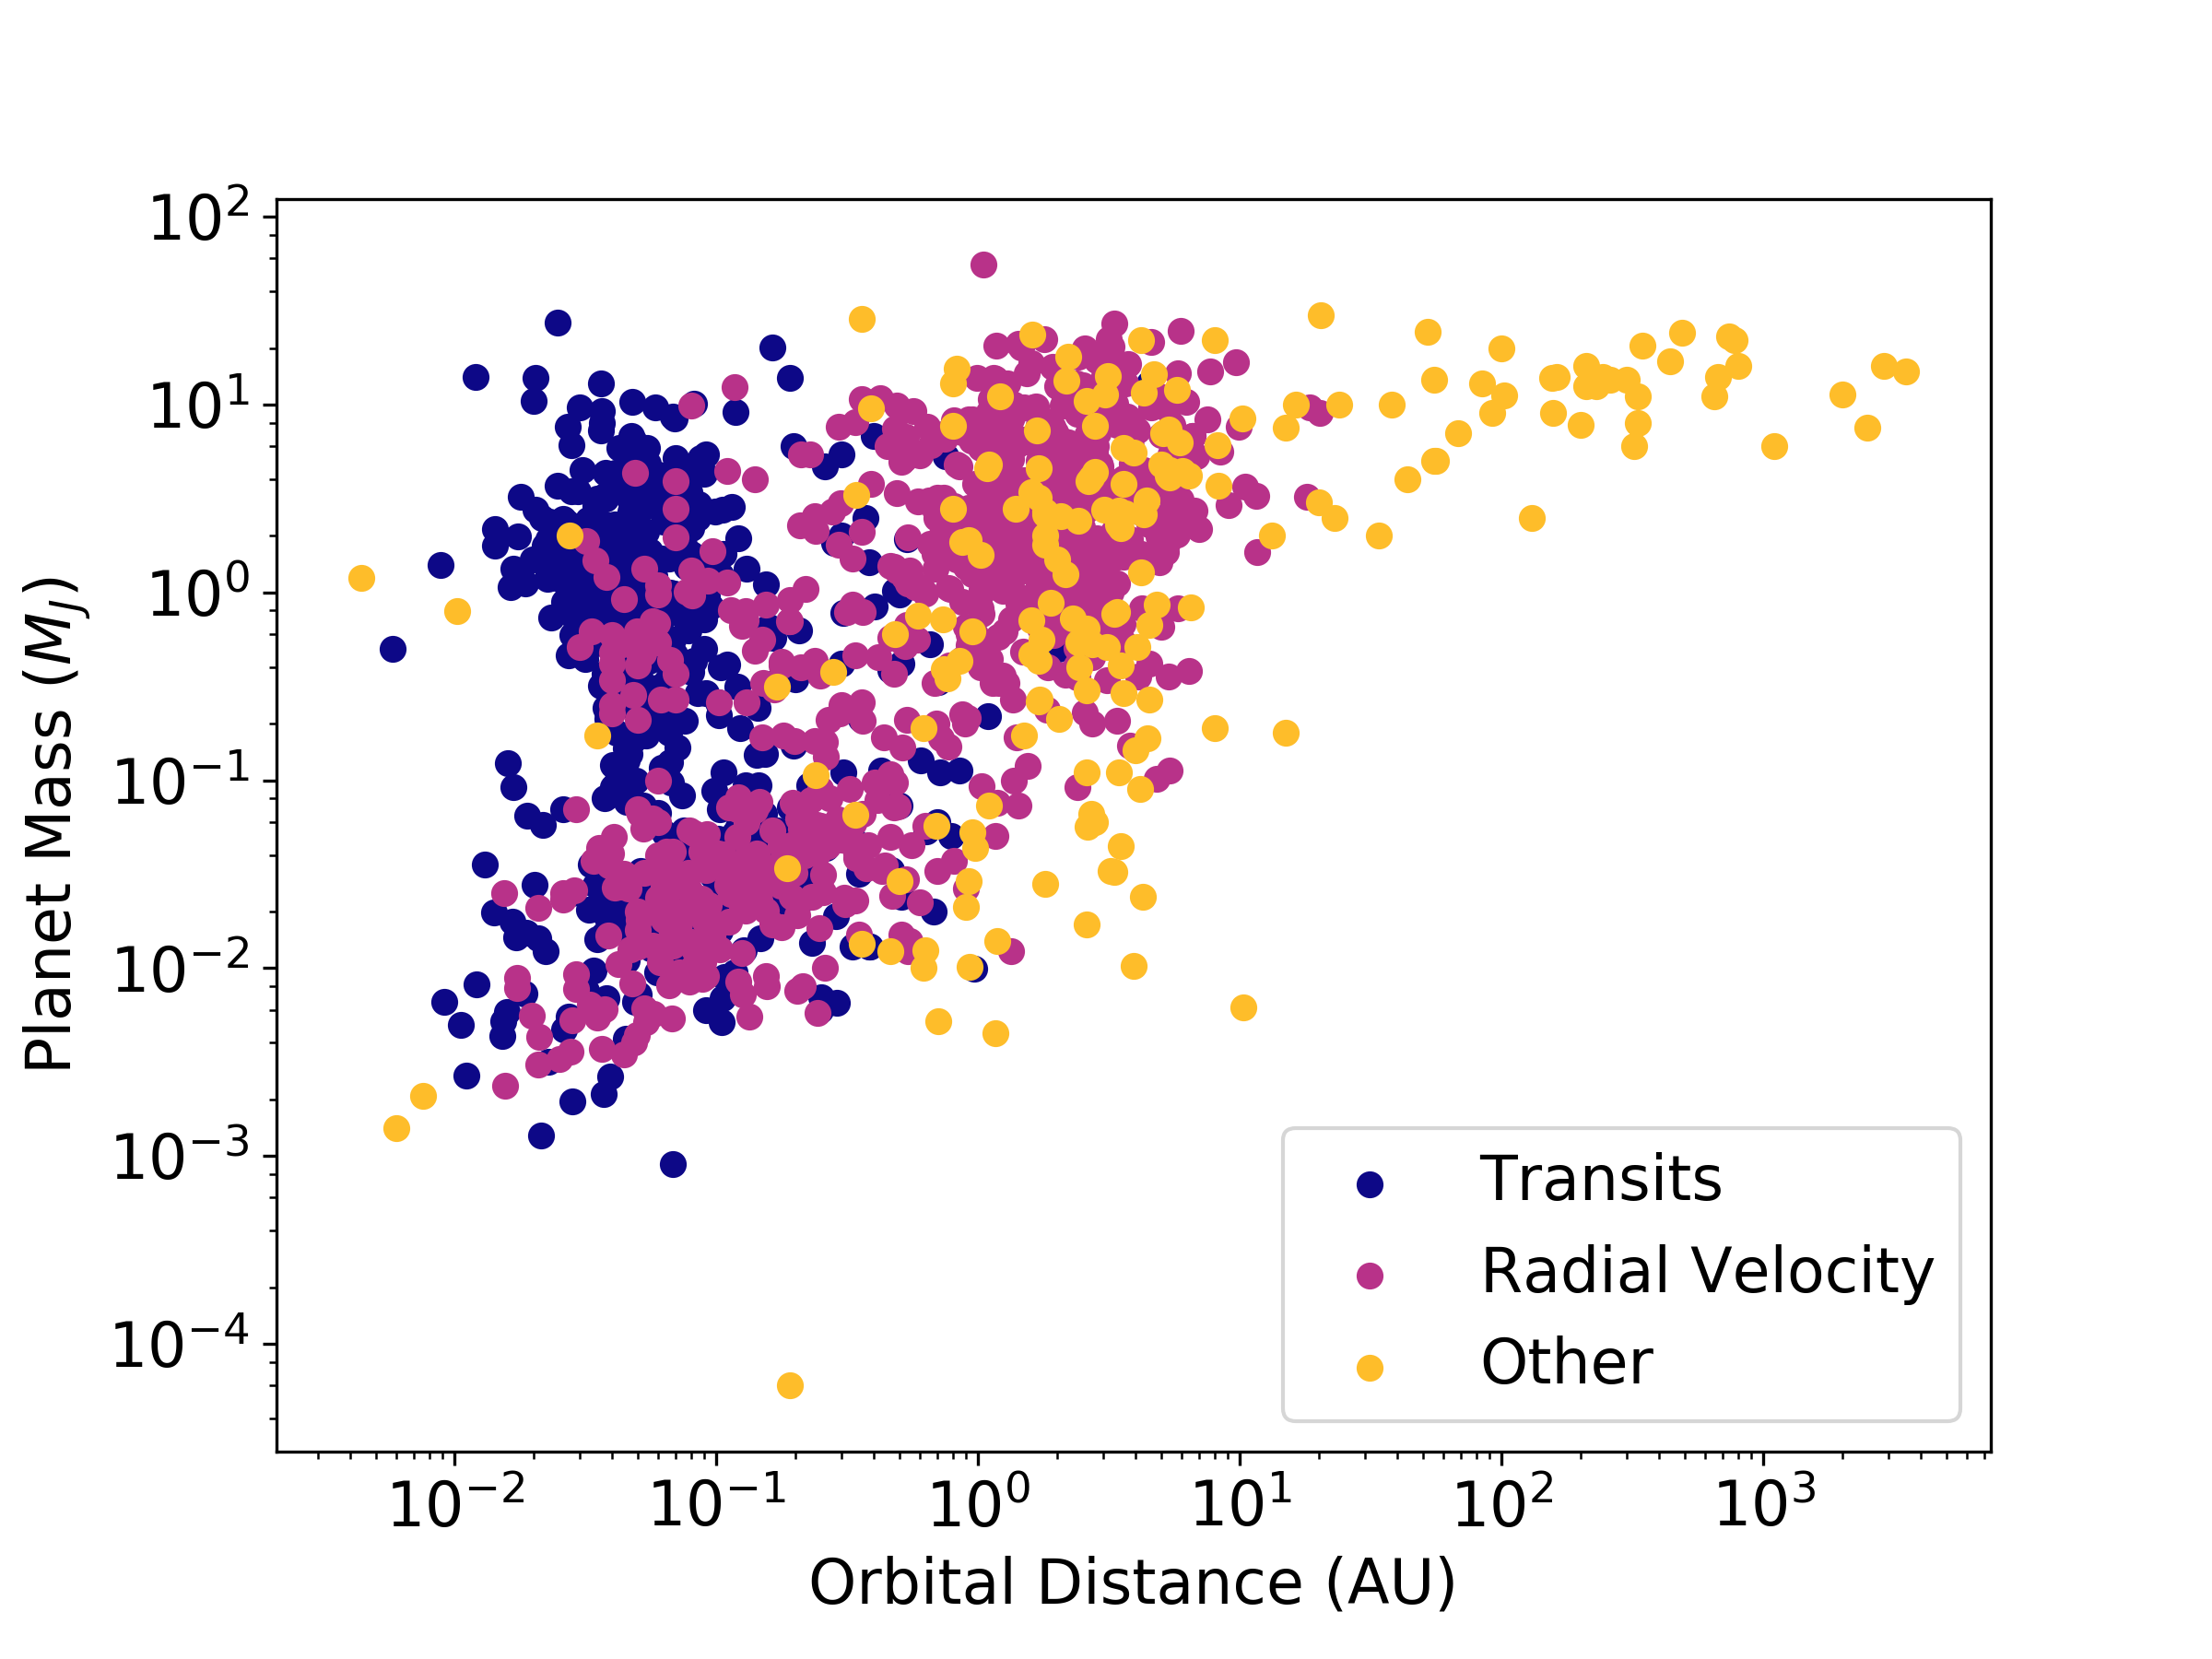
\includegraphics[width = \linewidth]{MA_NASAexo.png}
    \caption{Mass of the planet (or minimum mass for radial velocity planets) in Jupiter masses against the orbital distance in astronomical units for all of the confirmed exoplanets (4388 planets as of 1st June 2021, NASA Exoplanet Archive). Colors show the discovery methods: blue is transiting planets, purple is radial velocity detections and orange is all other detection methods.}
    \label{int:fig:ma}
\end{figure}

% Transit                          3306
% Radial Velocity                   823
% Microlensing                      106
% Imaging                            51
% Transit Timing Variations          21
% Eclipse Timing Variations          16
% Pulsar Timing                       7
% Orbital Brightness Modulation       6
% Pulsation Timing Variations         2
% Astrometry                          1
% Disk Kinematics                     1

On average, 50\% of the stars in our galaxy host at least one planet \citep{Howard2012,Dressing2013,Batalha2013,Silburt2015}. The 4,388 exoplanets confirmed to date range from small rocky planets to large gas giants. Figure \ref{int:fig:ma} shows a plot of mass vs orbital distance of all these planets colour-coded by discovery technique. Out of the many methods employed, two account for the vast majority of discoveries: transiting planets (3333 planets, shown in blue) and radial velocity planets (841 planets, coded purple).

Transiting planets pass in front of their star and create a periodic shadow in the flux measured from their star. The dimming of the stellar light when the planet passes in front of the star has a characteristic depth. This depth is a measure of the radius of the planet relative to the radius of the star (\rprss). On the other hand, radial velocity planets are detected by observing a signature of the movement of the host star due to the gravitational pull throughout the planetary orbit. Other techniques - represented by the colour orange in Figure \ref{int:fig:ma} - include microlensing, imaging, transit/eclipse timing variations, and pulsar timing.

The exoplanet population can be broadly classified into four families according to mass. At the lower end of the mass spectrum are the terrestrial planets, similar to the four smallest planets of our solar system: Mercury, Venus, Earth and Mars. Within this group fall  exoplanets with masses similar to the mass of Earth (around 0.5-2 $M_\oplus$ and sometimes even smaller). The second family are the Super-Earths. These planets are more massive than Earth (1 $M_\oplus = 3.1\times10^{-3} M_J$) but less massive than Uranus or Neptune and orbit their host stars at distances shorter than that between Earth and the Sun. Terrestrial planets and Super-Earths occupy the bottom left cluster of Figure \ref{int:fig:ma}. Super-Earths are considered the most abundant in our galaxy \citep{Borucki2011,Howard2012,Morton2014,Batalha2014,Petigura2013a,Petigura2018,Fulton2017,Bryson2020}. Rocky planets on short period orbits close to their host stars are known as hot-rocks or lava planets. They are so hot that their surface is mostly or entirely covered by lava oceans \citep[e.g.,][]{Leger2011, Elkins-Tanton2012, Winn2018}.

The third family is the Neptunian exoplanets, with masses similar to those of Neptune and Uranus. These are planets with rocky cores and  hydrogen/helium-dominated atmospheres. Warm-Neptunes (2-6$M_\oplus$ on short orbital periods) are a ubiquitous outcome of planet formation, occurring around more than 25\% of all stars \citep[e.g.,][]{Buchhave2014, Fulton2017}.

Finally, the largest exoplanets have masses similar to that of Jupiter. Due to their size, these planets are the easiest to find with current detection techniques. However, in absolute numbers, they are less common as other types of planets \citep[e.g.,][]{Gould2006,Howard2012,Fressin2013,Santerne2012,Wright2012}. Cooler Jupiter-like planets (top right cluster of Figure \ref{int:fig:ma}) are predominantly discovered by radial velocity and are ideal targets for direct imaging. In contrast, hot Jupiters (top left cluster of Figure \ref{int:fig:ma}) are mostly discovered by the transit method. Hot Jupiters are, as the name suggests, a similar mass to Jupiter but are on orbits that lie within the orbit of Mercury and so receive much more insolation from their host stars. As a result, their temperature is typically more than 1500K (1200$^\circ$C).  It is these gas giant planets that are the focus of this thesis.

% Aside from these main groups, there are also rocky planets smaller than super-Earths, some are on extremely short orbits, and these are dubbed the "hot-rocks". There are also ice giants like Neptunes or sub-Neptunes and smaller gas giants like Saturn or sub-Saturn type planets.

\subsection{The strength of the multiple system planets: masses from TTVs}% ( a short section on TTVs)

Out of the 4,000+ exoplantes discovered to date, 1879 belong to 750 multi-planet systems. Gravitational interactions between planets in the same system cause the planets to deviate from Keplerian orbits. This means that the orbital period is no longer a constant value and thus the time between each transit (planet crossing the star) will vary. This phenomenon is called transit timing variation (TTV). TTVs are useful in many areas of exoplanet science \citep[e.g.,][]{Schneider2003, Agol2005, Holman2005}. For example, they have been used to infer the presence of a non-transiting planet in a system where at least one planet is transiting or to confirm that a transit signal is indeed due to a planet and not a false positive. Additionally, TTVs can be used for planet characterization by constraining the masses and other orbital elements \citep[e.g.,][]{Ballard2011, Holman2010, Carter2012}.

 The Kepler mission provided four years of almost continuous optical photometric observations of several hundred multi-planet systems. Several studies have used this data to constrain the parameters of the orbital dynamics and planetary masses. In Chapter \ref{TTVs} of this thesis, we follow up on four of these systems using multiple transit observations per planet. We aim to confirm the TTV signal at another wavelength (near infrared with \spitzerIRAC compared to optical with Kepler) to lengthen the baseline of the previous Kepler observations and to look for signatures of more planets.

\section{Exoplanet atmospheres}
\subsection{Methods for probing exoplanet atmospheres}% (Look at Jacob’s 1.2)

There are two main methods for characterizing the atmospheres of exoplanets: direct imaging and transmission/emission spectroscopy. These can both be performed at either high or low resolution.

The probability of a planet transiting is $R_s/a$, where $R_s$ is the stellar radius and $a$ is the planetary orbital distance \citep{Borucki1984}. This means that there is a very small fraction of the population of exoplanets that are viable for transmission spectroscopy. In theory, direct imaging can be used to observe the atmospheres of these non-transiting planets. However, directly imaging exoplanets is difficult since telescopes and observatories have to overcome the very high contrast ratios between the star and the planet. With the detectors quickly becoming saturated by the stellar flux, there is often not enough time to gather enough photons from the planet. Nevertheless, with state-of-the-art coronagraphic and adaptive optics systems, several exoplanets have been directly imaged \citep[e.g.,][]{Marois2008,Marois2010,Lagrange2010,Rameau2013,Kuzuhara2013}.

This thesis focuses on characterizing the atmospheres of transiting planets. The transit method is a common technique for discovering planets. The measured transit depth and eclipse depth are wavelength and atmospheric composition-dependent quantities so can also be used to observe and study the atmospheres of planets \citep[e.g.,][]{Seager2000a, Brown2001, Charbonneau2005, Deming2005a}. In Figure \ref{int:fig:phasecurve} we show a schematic of a planet orbiting a star, which includes the transit (the planet in front of the star), the eclipse (the planet behind the star), and this full observation is called a phase curve. These techniques can each be used to study the properties of planetary atmospheres, giving us different parts of the story each time.

\begin{figure}
    \centering
    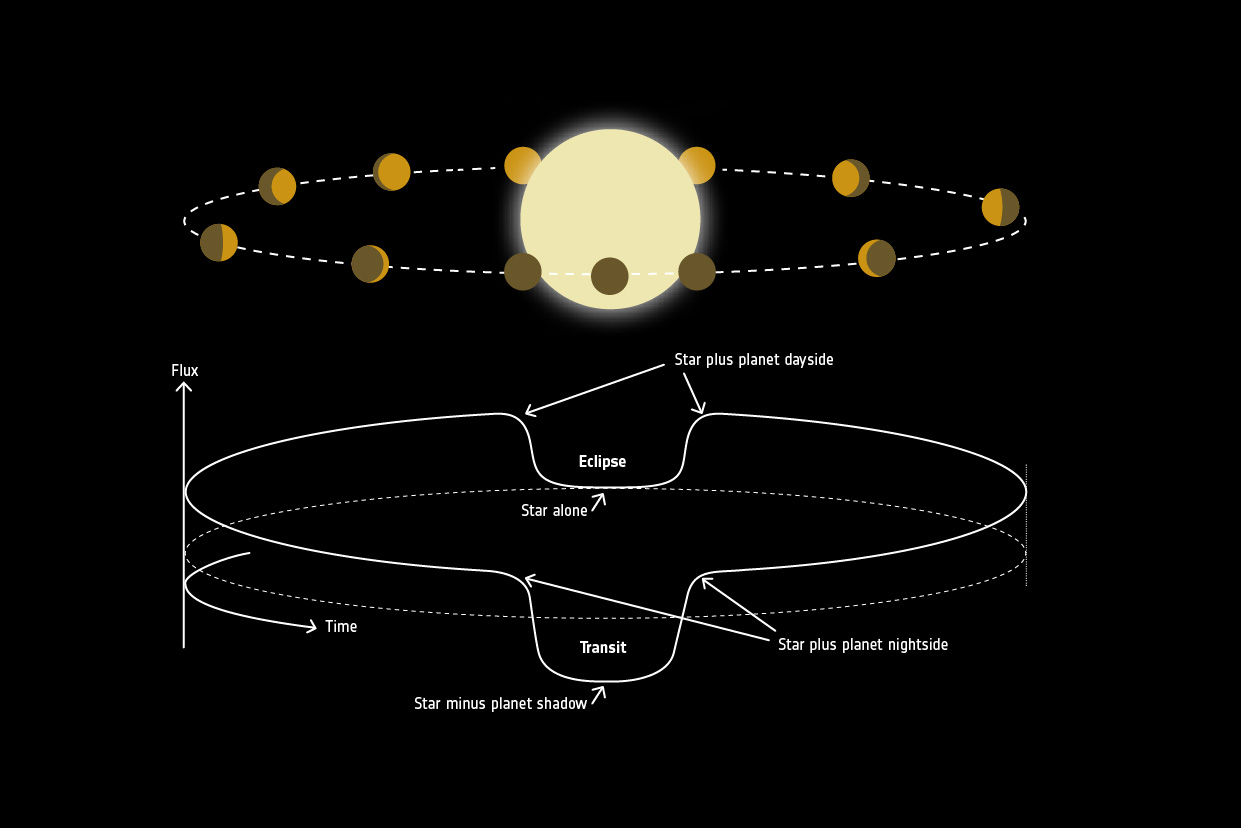
\includegraphics[width = \linewidth]{Exoplanet_phase_curve.jpg}
    \caption{Illustrative graphic detailing the full orbit of a planet around its host star, showing the transit and the eclipse. The full orbit observation is known as the phase curve, it captures all phases of the planet's tidally locked dayside. Image Credit: ESA}
    \label{int:fig:phasecurve}
\end{figure}

\subsubsection{Transmission spectroscopy}

The fractional change in the brightness of a star as a planet transits is equal to the radius of the planet divided by the radius of the star (\rprss). However, during the transit, a small fraction of the starlight passes through and is partially absorbed by the upper atmosphere of the planet. The strength of this atmospheric absorption is wavelength dependent due to the opacities of different molecular and atomic species. At wavelengths where the atmosphere is more opaque, the transit depth will be larger due to absorption of the stellar light, and where it is more transparent the transit depth will be smaller. Observing the planet transit across different wavelengths results in a transmission spectrum of the atmosphere. Transmission spectra can be compared with models of the chemistry and molecular opacities to gain insights into the atmospheric composition \citep{Charbonneau2002, Vidal-Madjar2003, Tinetti2007, Swain2008}.

Typically, differences in the transit depth are larger for hot, puffy atmospheres with large scale heights ($H$):

\begin{equation}
    H = \frac{k_B T}{\mu_m g},
\end{equation}

where $T$ is the temperature, $\mu_m$ is the mean molecular mass, $g$ is the gravitational acceleration and $k_B$ is Boltzmann's constant. The scale height is a measure of the increase in altitude when the atmospheric pressure decreases by a factor of $e$, and for hot Jupiter atmospheres is on the order of a few hundred kilometers. In many cases, we use the equilibrium temperature ($T_{\rm eq}$) for $T$ and the planetary surface gravity for $g$.

The measured difference in the transit depth (\rprss) resulting from an absorption feature can be written in terms of the number of scale heights crossed ($N_H$),

\begin{equation}
\Delta \delta = \frac{\pi(R_p + N_H H)^2}{\pi R_s^2} -
\frac{\pi R_p^2}{\pi R_s^2}
 \approx 2 N_H \delta \left(\frac{H}{R_p}\right).
\label{int:eq:NH}
\end{equation}

where $\delta$ is the transit depth (\rprss) and $\Delta\delta$ is the difference in the transit depth inside and outside a molecular feature. Hotter planets are expected to have larger atmospheric absorption signals ($\Delta\delta$), due to the dependence on $H$ which scales with the temperature. However, the technique of transmission spectroscopy has successfully been applied to cooler targets as well \citep[e.g.,][]{Desert2011b, Berta2012, Crossfield2017}. In Chapter \ref{transits} we use equation \ref{int:eq:NH} to determine how many scale heights the \spitzer Space Telescope probes on average between 3.6 and 4.5~\um~for a survey of 49 transiting planets ranging from 600 to 2600 Kelvin. %The mean scale height for this sample of planets is 550$\pm$330~km.
We show that, for our sample of planets, we probe an average of 0.5 scale heights between the two \spitzerIRAC bandpasses at the 7$\sigma$ level.

\subsubsection{Emission Spectroscopy}

The dayside emission of a planet can be measured by observing the planet before, during, and after it passes behind the star. Similar to the transit, this creates a dip in the light measured throughout time. The depth of that dip, or the eclipse depth, is a measure of the fractional flux of the planet relative to the star (\fpfs). Here, $F_p$ and $F_s$ are used to represent the disk-averaged spectral density multiplied by the disk area for the planet and the star respectively. The eclipse depth, in absence of any spectral features, can be represented by the ratio of two Planck functions multiplied by the transit depth,

\begin{equation}
\frac{F_p(\lambda)}{F_s(\lambda)} = \frac{B_\lambda(T_p)}{B_\lambda(T_s)}~\frac{R_p^2}{R_s^2},
\end{equation}

where $B_\lambda(T)$ is the Planck function,

\begin{equation}
B_\lambda(T) \equiv \frac{2hc^2}{\lambda^5} \frac{1}{e^{hc/(\lambda k_B T)} - 1}
\end{equation}

in which $T$ is the temperature of the planet or the star, $\lambda$ is the wavelength, $h$ is Planck's constant, and $c$ is the speed of light. Assuming the temperature of the star is known, this formulation can also be used to solve for the planetary temperature at a specific wavelength, this is known as the brightness temperature, $T_B$. In Chapter \ref{eclipses}, we calculate the brightness temperature of our planets by using stellar models instead of a blackbody for the star. Additionally, we incorporate the \spitzer spectral response functions and rigorously integrate the formulation over the bandpasses to accurately determine the brightness temperatures of a survey of planets with emission at 3.6 and 4.5~\um.

Unlike transmission spectroscopy, where the starlight is passing through the stellar atmosphere, emission spectroscopy measures the emission of the planet relative to the star. The emission spectrum of the planet will deviate from a blackbody depending on the atmospheric composition and temperature structure probed by the photons traveling through the atmosphere (see Section \ref{int:sec:TP} for more on the temperature structure). The crucial difference between the information gathered from transmission spectroscopy and emission spectroscopy is the depth probed in the atmosphere. Due to the slant geometry, an optical depth of 1 is reached at much lower pressures in transmission compared to the normal geometry in emission \citep{Fortney2005}. Therefore in general, transmission spectroscopy probes the upper more tenuous layers of the atmosphere at pressures around 1 millibar, whereas emission spectroscopy probes deeper layers at pressures of around 0.1-10 bar (depending on the wavelength).

\subsubsection{Phase curves}

A phase curve observation consists of observing the planet throughout its entire orbit, including the transit and the eclipse. Planets on close-in orbits of $\lesssim10$ days typically become tidally locked, with permanent day and night sides \citep[e.g.,][]{Guillot1996}. Therefore, a phase curve allows us to observe the planet as a function of its rotational phase, as demonstrated in Figure \ref{int:fig:phasecurve}. At each orbital phase, different longitudes of the planet's dayside are rotating into the view of the observer. The difference in brightness between any two points in phase can be used to reconstruct a brightness map of the planet's surface \citep{Knutson2007, Knutson2012, Crossfield2012, Borucki2009, Snellen2009}. At optical wavelengths, the planetary brightness is dominated by reflected light from the star, and so a phase curve observation provides constraints on the planet's albedo. On the other hand, at infrared wavelengths, the planetary brightness is dominated by thermal emission, resulting in longitudinal information about the planet temperature \citep{Parmentier2018b}.

As well as the eclipse depth (\fpfs) and the transit depth (\rprss), a phase curve observation can provide us with the measurement of the maximum flux, the phase of the maximum flux relative to eclipse (known as the phase curve offset), and the relative amplitude of the phase curve (day-to-night temperature contrast). Since these planets are tidally locked, the substellar point is brighter than the limbs of the planet. This brightest point can lag (negative offset, westward shift) or lead the substellar point (positive offset, eastward shift). These shifts are measured with the phase curve offset as well as the day-to-night temperature contrast \citep{Showman2002}. Parameterizing the phase curve like this is useful for studying the energy balance and the dynamics of the atmosphere \citep{Cowan2012b, Schwartz2015}. In Chapter \ref{eclipses}, we use the phase curve offset measured in each of the two \spitzerIRAC bandpasses to determine if a measurement of the efficiency of redistribution from eclipses will change over the two wavelengths.

Similar to transits and eclipses, these phase curves can be measured spectro-photometrically or spectroscopically. At the wavelengths with a strong opacity source and strong atmospheric absorption, a phase curve probes higher in the atmosphere (at low pressures), whereas outside an absorption band the phase curve observation probes deeper (high pressures) \citep{Showman2009, Kataria2015}. This technique allows for maps of the chemistry and temperature structure and a map of the flux and brightness temperature \citep{Cowan2008, Showman2008, Knutson2009c, Stevenson2017}. Furthermore, \citet{Arcangeli2021} measured the first emission spectrum at quadrature without the need to observe a full phase curve observation of WASP-12b.

\subsection{Instrumentation for probing exoplanet atmospheres used in this thesis} %(your previous 2.2)

This thesis mainly focuses on using multi-epoch observations of exoplanet atmospheres in emission and transmission in the two photometric bandpasses of the \spitzer Space Telescopes Infrared Array Camera (\spitzerIRAC) \citep{Werner2004}. However, in Chapter \ref{eclipses} we expand on our work with \spitzer by studying full emission spectra taken with the Hubble Space Telescope Wide Field Camera 3 (HST/WFC3) to compare the effects of atmospheric properties at different wavelengths and depths in the atmosphere. Both of these telescopes are space-based observatories, which are advantageous over ground-based observatories as they offer both stability and sensitivity while bypassing the Earth's atmosphere. This is especially  important for this work because the atmosphere of the Earth absorbs in the infrared where there are absorption signatures of the particular  molecules that we study, such as water vapor and carbon dioxide.

\subsubsection{\spitzerIRAC}

Launched in 2003, \spitzer Space Telescope was cryogenically cooled with liquid helium cryostat to 15K and could observe between 3 and 24~\um~over four photometric bands with the Infrared Array Camera \citep[IRAC,][]{Fazio2004}. In 2009, \spitzer exhausted its supply of liquid helium and entered the post-cryogenic mission, so called ``Warm-\spitzer'' at $\sim$30K \citep{Mcmurtry2006}, with just the two shorter wavelength bands remaining active, 3.6 and 4.5~\um. After 16 years of observations, the \spitzer Space Telescope was decommissioned on the 30th of January 2020. Nevertheless, there remains a wealth of knowledge available from the archival data, which is a focus of this thesis. The two remaining wavelength bands of \spitzerIRAC mainly capture the atmospheric signatures of methane (\ce{CH4}), carbon monoxide (\ce{CO}), carbon dioxide (\ce{CO2}), and water (\ce{H2O}). In Chapters \ref{transits} and \ref{eclipses} we show the atmospheric opacities of the molecules probed with \spitzerIRAC in emission and transmission respectively.

\subsubsection{HST/WFC3}

The Hubble Space Telescope contains some of the current best instruments for measuring the atmospheres of exoplanets. The Wide Field Camera 3 (WFC3) is capable of measuring spectra from 0.8 to 1.7~\um~with two separate grisms. In Chapter \ref{eclipses} we use the emission spectra measured with the WFC3/G141 grism, which captures the 1.4~\um~water feature. We combine these observations with our \spitzerIRAC photometry.

\subsection{Systematics and Noise Sources}

When attempting to measure the precise signal of an exoplanet atmosphere, dealing with the various noise sources becomes very important. The first noise source is unavoidable: photon noise or shot noise. Each atom inside the star emits a photon with some probability, this probability follows a Poisson distribution with a standard deviation of $\sqrt{N}$, where $N$ is the number of events or counts detected. The other noise sources to correct for are the background noise, dark current, and readout noise. Background noise is the incoming light on the detector in the absence of any apparent sources (e.g. zodiacal light). Dark current arises from thermal fluctuations in the electrons of the detector. Readout noise is the amount of noise generated from the electronics itself, it is a similar contribution to the background noise for \textit{Spitzer}. In our analysis of Spitzer lightcurves (first presented in Chapter \ref{transits}) we measured and subtracted the background from our observations using several different techniques and determined which was the best for each planet.

\subsubsection{\spitzerIRAC intrapixel sensitivity}

\begin{figure}
    \centering
    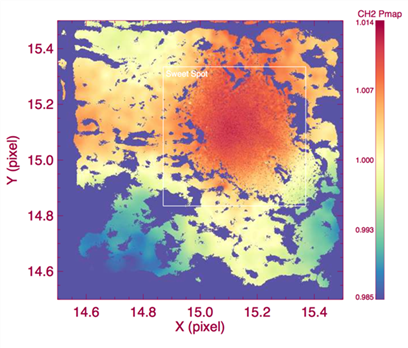
\includegraphics[width = \linewidth]{IRAC_Instrument_Handbook183.png}
    \caption{Map of the intrapixel sensitivity of the central pixel on the detector at 4.5~\um~ for warm-\spitzerIRAC data. The x and y axis show the fraction of the central pixel and the colour map shows the pixel sensitivity with red showing a higher sensitivity. Image Credit: \spitzerIRAC Instrument Handbook\footnote{https://irsa.ipac.caltech.edu/data/\spitzer/docs/irac/iracinstrumenthandbook/47/}.  }
    \label{int:fig:pmap}
\end{figure}

Each instrument that exoplanets scientists currently use has a set of challenges regarding detecting the signals of exoplanet atmospheres since none of these facilities were designed with exoplanet characterization in mind. The most important and strongest instrumental effect that we need to account for with \spitzer data is the gain variations within a single pixel, known as the intrapixel sensitivity effect. Figure \ref{int:fig:pmap} demonstrates the photometric gain at 4.5~\um~of the central pixel of the \spitzerIRAC detector. The target moves across the detector due to the following effects: a settling drift after slewing, a long-term drift due to an inconsistency in velocity corrections, jitter, and a thermally induced oscillating pointing drift due to periodic on-off cycling of the battery heater within the spacecraft. This movement in combination with the changes in gain causes temporal variations in the amount of flux measured from a constant source. The typical signature of a few scale heights in the atmosphere of a hot Jupiter is about 100 parts per million (0.1\%). The amplitude of the intrapixel variations seen in \spitzer lightcurves is on the order of 1\%. Thus, we need to accurately correct these systematics to obtain the precision required to detect atmospheric signatures.

We typically overcome the settling drift by having a peak-up throw-away observation of about half an hour and by discarding $\sim$15 minutes from the beginning of the observation. Next, we model the long-term settling drift with a linear function of time. There have been many efforts over the years to model and correct the periodic systematics induced from the pointing variations \citep[e.g.,][]{Charbonneau2008,Ballard2010, Knutson2012,Stevenson2012, Evans2015, Morello2015a, Morello2015b, Buzasi2015, Deming2015, Krick2016}.

% \begin{itemize}
% \item Polynomial fitting \citep{Charbonneau2008}
% %\item MCMC Evaluation \citep{Gillon2010}
% \item Kernel Regression Mapping, using the data to be corrected \citep[KR/Data;][]{Ballard2010, Knutson2012}
% \item BiLinearly Interpolated Subpixel Sensitivity \citep[BLISS;][]{Stevenson2012}
% \item Gaussian Process Models \citep[GP;][]{Evans2015}
% \item Independent Component Analysis \citep[ICA;][]{Morello2015a, Morello2015b}
% \item Segmented Polynomial for the K2 Pipeline \citep[SP(K2);][]{Buzasi2015}
% \item Pixel Level Decorrelation \citep[PLD;][]{Deming2015}
% \item Kernel Regression using a calibration pixel mapping dataset \citep[KR/Pmap;][]{Krick2016}
% \end{itemize}
All of these different methods culminated with a repeatability and reliability data challenge, the results of which were presented in \citet{Ingalls2016}. Each of the methods were tested on ten real and ten simulated eclipses of XO-3b. The data challenge found that most of the methods were able to estimate accurate uncertainties on individual eclipses. However, they found that BiLinearly Interpolated Subpixel Sensitivity \citep[BLISS;][]{Stevenson2012}, Pixel Level Decorrelation \citep[PLD;][]{Deming2015}, and Independent Component Analysis \citep[ICA;][]{Morello2015a, Morello2015b} were the most accurate and repeatable for correcting systematics on observations of large pointing fluctuations. Furthermore, they found that PLD was also able to obtain the highest accuracy on a the simulated dataset. In this thesis, we focus on using PLD \citep{Deming2015}, while also testing the original polynomial fitting \citep{Charbonneau2008} as well as Gaussian Process models \citep[GP;][]{Evans2015}.

\subsubsection{Pixel Level Decorrelation}

Unlike several of the other techniques, Pixel Level Decorrelation \citep{Deming2015} does not require knowledge of the sub-pixel position or a map of the variations in the sub-pixel sensitivity. Instead, it assumes that the flux from the star will be a smooth function of position, such that when the target moves on the detector, the neighboring pixels will receive more or less flux depending on if the target is moving towards or away from the pixel in question. The sub-pixel position is therefore encoded implicitly in a generalized function of pixel intensity. Such a smooth function can be differentiated and can also be Taylor expanded. Doing this allows us to model the flux in time as a weighted sum of individual pixel fluxes. To model the full photometric lightcurve in time ($t$) we combine the weighted pixel flux sum with a transit or eclipse model ($TD(t)/ED(t)$) and a linear slope in time ($ft$) to model the long-term drift:

\begin{equation}
    \Delta S^t = \sum_{i=1}^{N}c_i \hat{P}_i^t + TD(t) + ft,
\end{equation}

where $S^t$ is the flux measured over time and $\Delta$ represents the total fluctuations from all sources. $\hat{P}_i^t = \frac{P_i^t}{\Sigma_{i=1}^{N}P_i^t}$ represents the normalized flux from pixel $i$ at time $t$, where a grid of $i$ pixels are chosen around the centroiding position.

\subsection{Properties and Climates of exoplanets}%  (look at Arcangeli section 1.3)

\subsubsection{Chemistry}

Since hot Jupiters are gas giants, their atmospheres are primarily composed of gaseous Hydrogen and Helium \citep{Seager1999}, with most of their other constituents also being in gas phase, such as water, methane, carbon monoxide and carbon dioxide \citep{Brown2001}.

A typical assumption when modeling atmospheres is that the chemical composition of the atmosphere is the same as our Sun (solar composition): 74.9\% Hydrogen and 23.8\% Helium, with all the heavier elements (which are known as \textit{metals} in astrophysics) encompassing the other 1.3\%. Starting from this assumption, a series of chemical networks are used to calculate the abundances of molecular species in the atmosphere. A common assumption for these chemical networks is that the atmosphere is in chemical equilibrium, meaning that the molecular abundances can be determined, in the first order, from the temperature and pressure alone. Under these assumptions, predictions can be made about which molecules would be expected to be abundant for different temperatures of planets.

\spitzer is an invaluable tool to test these assumptions because it is sensitive to the abundance of methane, water, carbon monoxide and carbon dioxide (\ce{CH4} and \ce{H2O} at 3.6~\um~and \ce{CO}, \ce{CO2}, \ce{H2O} at 4.5~\um). The strength of the \ce{H2O} opacity is approximately equal in both \spitzerIRAC bandpasses (see Figure 1 of Chapter \ref{eclipses})/ Therefore, \spitzer can be used to probe the relative abundance of CO and \ce{CH4} \citep{Madhusudhan2019}. Since these are both carbon-bearing species, and since carbon (C) is less abundant than hydrogen (H) and oxygen (O), there is a trade-off between CO and \ce{CH4} with temperature. The following summary chemical reaction arising from the \ce{CH4}-CO conversion reaction scheme plays an important role in determining the dominating carbon-bearing species in an atmosphere \citep[e.g.,][]{Visscher2010, Moses2011, Visscher2011}:
\\
\\
\ce{ \centering CH4 + H2O <=> CO + 3H2}.
\\
\\
For a nominal pressure of 1 bar, temperatures higher than $\sim$1100~K favor \ce{CO} creation, and lower temperatures favor \ce{CH4} creation \citep[e.g.][]{Madhusudhan2012, Molliere2015, Molaverdikhani2019}. Therefore, hotter planet atmospheres are predicted to have carbon monoxide and cooler planets are predicted to have methane as the dominant carbon-bearing species, with the transition occurring at around 1100K, depending on the pressure being probed (emission probes deeper than transmission).

In reality, there are several phenomena that can cause an atmosphere to deviate from equilibrium: photochemistry, vertical mixing, higher metallicity, cloud/haze formation, tidal heating, winds, and other dynamical interactions \citep[e.g.,][]{Madhusudhan2019}. In Chapter \ref{transits} we study the effects of some of these processes by modeling them and comparing several different grids of models to a survey of 49 planets in transmission.


\subsubsection{Temperature structure}
\label{int:sec:TP}

\begin{figure}
    \centering
    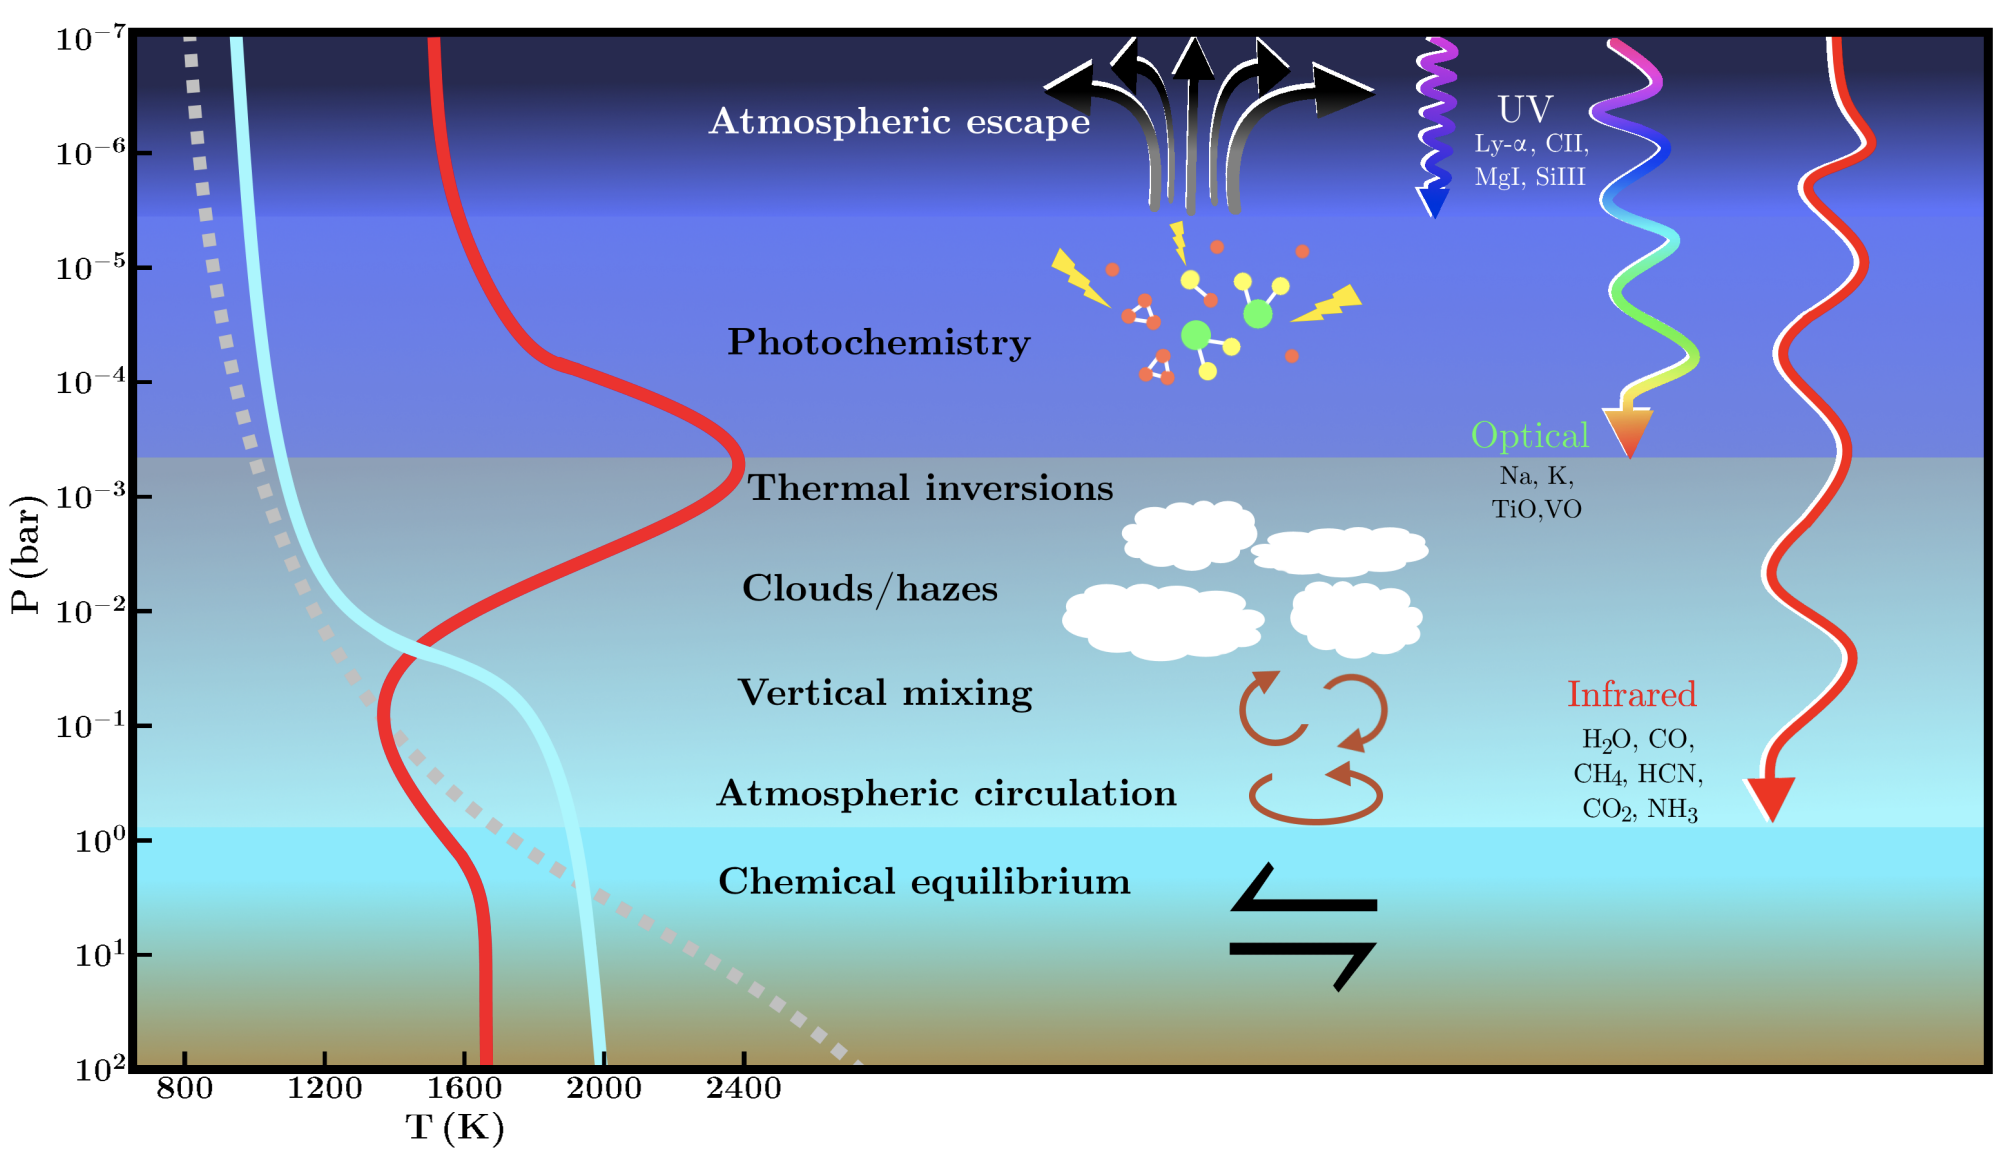
\includegraphics[width = \linewidth]{TPandeffects.png}
    \caption{Properties and processes active in the atmospheres of exoplanets. On the left and 3 model temperature-pressure profiles: grey-dashed is that of a non-irradiated atmospheres, cyan is an irradiated atmospheres with a nominal temperature-pressure profile and red is a highly irradiated atmosphere with a temperature inversion. Image Credit: \citep{Madhusudhan2019}}
    \label{int:fig:TPs}
\end{figure}

Just like on Earth, the temperature of a hot Jupiter atmosphere does not remain constant with altitude, i.e., it is not isothermal. Typically, the atmosphere gets hotter towards higher pressures. The gray dashed line in Figure \ref{int:fig:TPs} shows a typical temperature-pressure profile (TP) of a model atmosphere. In the deep atmosphere, at high pressures, the atmosphere is opaque and the energy is therefore transported convectively via bulk movement of gas. This results in inefficient transport and a large temperature gradient. Whereas in the upper more tenuous atmosphere, energy is transported radiatively which is a more efficient process, resulting in less steep temperature gradients.

The cyan line in Figure \ref{int:fig:TPs} shows an irradiated atmosphere with a nominal (non-inverted) temperature-pressure profile. The red line shows that of a highly irradiated atmosphere with a temperature inversion. A temperature inversion is where the temperature starts to increase with decreasing pressure. This is caused by the UV/visible absorption of the strong incident stellar irradiation, leading to the heating of the upper layers of the atmosphere. Earth's stratosphere contains a thermal inversion due to the absorption of Ozone (\ce{O3}). In hot Jupiters, molecules such as titanium oxide (\ce{TiO}) and vanadium oxide (\ce{VO}) are thought to be the cause of their thermal inversions \citep{Hubeny2003, Fortney2008, Desert2008}. Additioanlly, recent work has also suggested that temperature inversions in ultra-hot Jupiters may be caused by the absorption of metals and metal hydrides \citep[Fe, Mg, SiO][]{Lothringer2018} or other metal-rich species \citep[AlO, CaO, NaH and MgH;][]{Gandhi2019}.

The detection of molecular features in exoplanet atmospheres via emission spectroscopy not only tells us about the atmospheric chemistry on the dayside but it is also a probe of these vertical temperature profiles. For a nominal temperature-pressure profile (temperature decreasing with altitude), if a molecule is present and has an opacity at the wavelength of observation, then it will absorb the radiation and the measured eclipse depth will be smaller than the continuum. For example, Figure \ref{int:fig:w43} shows an HST/WFC3 spectroscopic observation from \citet{Stevenson2014c} where the 1.4~\um~water absorption feature can be seen clearly in the emission spectrum. The temperature-pressure profile retrieved for the dayside of WASP-43b is very similar in shape to the diagram of an irradiated atmosphere in Figure \ref{int:fig:TPs}.

For an inverted TP profile, a molecule will emit radiation at a temperature higher than the continuum and so the eclipse depth will appear larger at the wavelength of the opacity. Figure \ref{int:fig:w18} shows an emission spectrum of WASP-18b, where you can see the 4.5~\um~CO feature appearing in emission due to the temperature inversion. There have been a few studies finding evidence for temperature inversions in hot and ultra-hot Jupiters \citep[e.g.,][]{Knutson2008,Knutson2009b,Madhusudhan2010,Haynes2015,Evans2017,Arcangeli2018}. However, some of the early observations were revised \citep[e.g.,][]{Diamond-Lowe2014}. Temperature inversions were notoriously difficult to establish in the available observations of hot Jupiters. In Chapter \ref{eclipses} we use our sample of planets in emission with \spitzerIRAC observations to statistically measure a transition from the hot Jupiters to the ultra-hot Jupiters which is likely due to temperature inversions, among other effects.

\begin{figure}
    \centering
    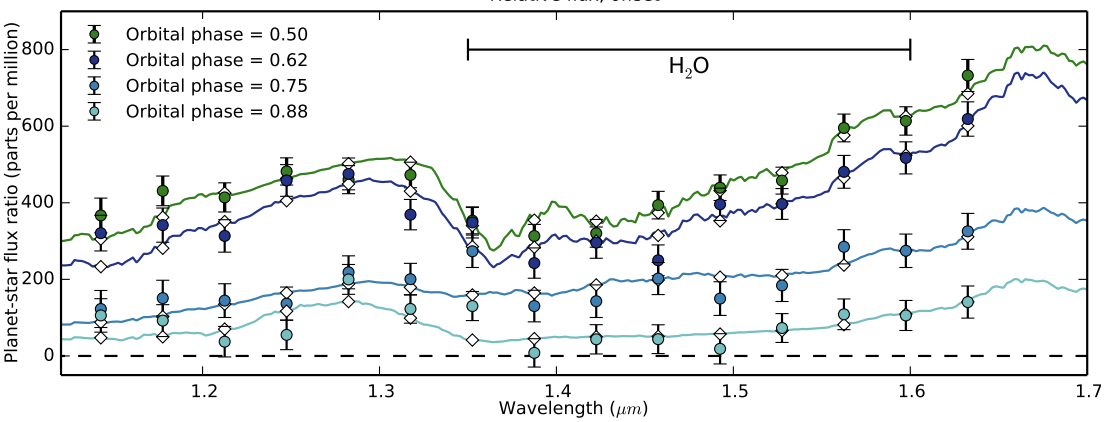
\includegraphics[width = \linewidth]{Wasp-43b_water.png}
    \caption{Emission spectrum of WASP-43b taken from a spectroscopic phase curve observation. Green data and model shows the emission spectrum during phase 0.5, which is what would be observed with an eclipse only observation. This clearly shows the water absorption feature appearing due to a nominal temperature-pressure profile. Other lines show the planet as it approaches quadrature (phase 0.75). At quadrature, you are observing half of the dayside and half of the nightside. Image credit: \citet{Stevenson2014c}.}
    \label{int:fig:w43}
\end{figure}

\begin{figure}
    \centering
    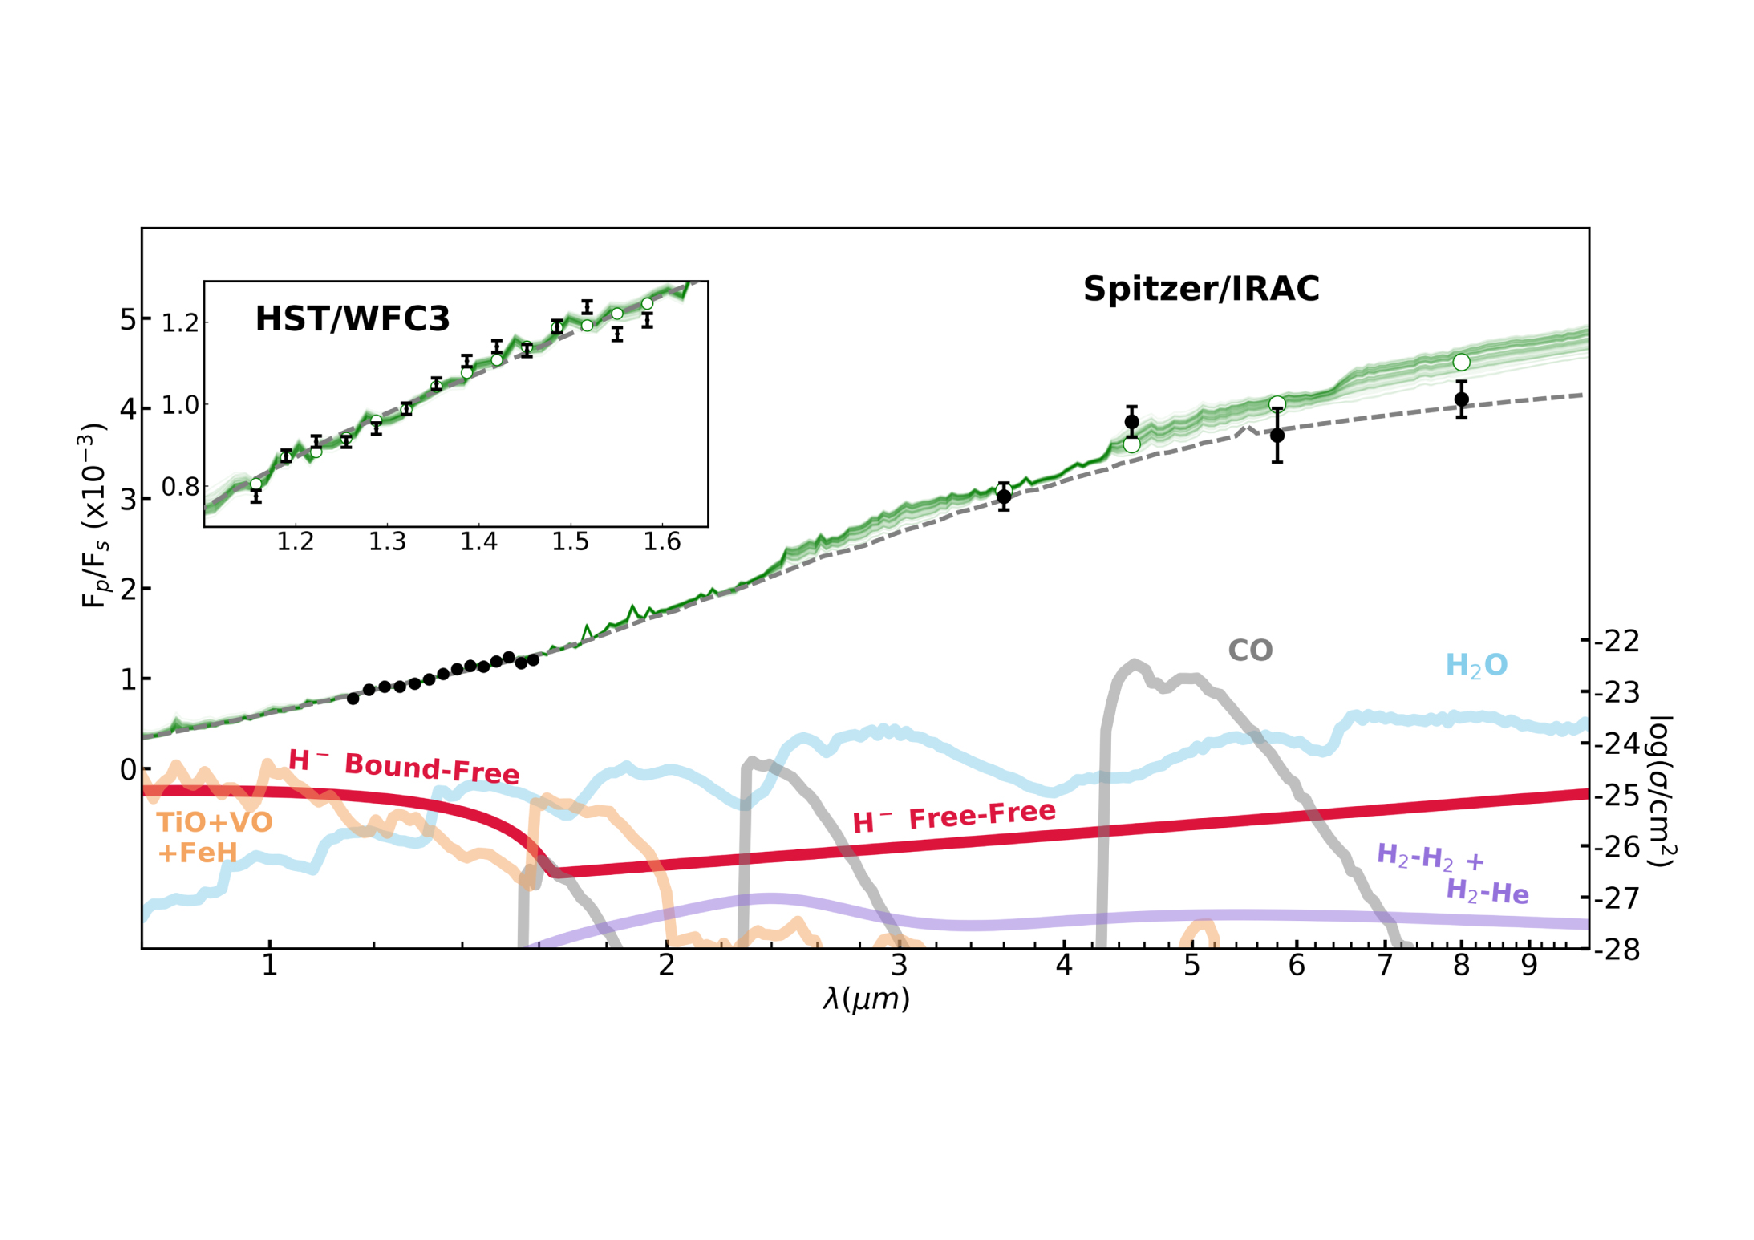
\includegraphics[width = \linewidth]{arcangeli+18.pdf}
    \caption{Emission spectrum of WASP-18b from HST and Spizter/IRAC (black data points). Green lines show the retrieved models, and the cross-sections of the important opacity sources are shown on the bottom of the Figure. The 4.5~\um~ \spitzer eclipse depth shows the CO feature appearing in emission due to the temperature-pressure profile. At the HST/WFC3 wavelengths, we see that the combination of \ce{H2O} and H- bound free opacity makes the emission appear like a blackbody. Image credit: \citet{Arcangeli2018}. }
    \label{int:fig:w18}
\end{figure}

Figure \ref{int:fig:TPs} also shows the pressure levels where several physical processes occur in planetary atmospheres. Each of these processes is also inexorably intertwined with the temperature-pressure structure, but we will discuss some of them individually in the following sections.

\subsubsection{Clouds and hazes}

This thesis focusses on the study gas giant exoplanets ranging from those cooler than the Earth \citep[Kepler-16b, 200K;][]{Doyle2011} all the way to the hottest ultra-hot Jupiter \citep[KELT-9b, 4000K;][]{Gaudi2017}. It is expected that somewhere in this range of temperatures, aerosols will form. Aerosol is the all-encompassing term for clouds, hazes, and dust. Clouds are particles forming in the atmospheres as a result of first order phase changes. Due to the temperature-pressure profile crossing a condensation curve of some molecule, e.g., gas to liquid water. Cloud formation can also occur as a result of thermochemical reactions. On the other hand, haze formation can be defined as the formation of particles via the breakdown of molecules due to energy input e.g., photochemistry of energetic particle bombardment. Both clouds and hazes have the effect of dampening the atomic and molecular signatures seen in the atmospheres of exoplanets, sometimes making the transmission spectra appear mostly flat in the visible and near-infrared wavelenths \citep[e.g.,][]{Charbonneau2002, Fortney2003, Pont2008}.

Even in our own solar system, aerosol composition is extremely diverse: from water on Earth, sulfuric acid on Venus \citep{Hansen1974}, ammonia on Jupiter and Saturn \citep{Brooke1998, Baines2009} and many different complex organics and hydrocarbons on the outer solar system planets and moons \citep[e.g.,][]{Sromovsky2011, Romani1988, Sagan1992, Brown2002, Rages1992}. Aerosols were therefore predicted to be found in the atmospheres of exoplanets. In fact, the very first transmission spectrum of an exoplanet showed dampening of the predicted absorption feature by atomic sodium in the atmosphere of HD 209458b. One of the possibilities that could account for the reduced sodium abundance was the presence of high altitude aerosols \citep{Charbonneau2002}. Given equilibrium chemistry, different molecules/elements will condense to form clouds at different pressures \citep{Lodders2004, Marley2013}. This depends on when the temperature-pressure profile of the atmosphere crosses the condensation curves of the cloud forming species.
%Additionally, different molecules will be abundant in the atmospheres of planets of different temperatures, so different cloud layers are expected to form in planets of certain temperatures \citep{Marley2013}.

% transmission spectra
% emission spectra
% reflected light

As well as dampening molecular features in transmission spectra, clouds can leave their own spectral fingerprint. In particular, high altitude \ce{H2} particles create a Rayleigh scattering slope in the transmission spectra
%. Rayleigh scattering is the elastic scattering of light by particles, the intensity of light scattered by a particle goes as 1/$\lambda^4$ meaning that smaller wavelengths (bluer light) scatter more than longer wavelengths (redder light). This causes the transit depth to be deeper towards the blue part of the electromagnetic spectrum, creating the typical Rayleigh slope seen by observers
\citep[e.g.,][]{LecavelierdesEtangs2008,Sing2015, Sing2016, Gibson2017}. Similarly, clouds can plague our observations and leave spectral signatures via Mie scattering \citep[e.g.,][]{Benneke2019} or their own absorption features \citep[e.g.,][]{Wakeford2015}. It is hoped that in the future, the James Webb Space Telescope will be used to pin down the composition of aerosols using computations of possible cloud species in combination with the observations \citep[e.g.,][]{Gao2020}.

\subsubsection{Dynamics, climate and variability}

\label{int:sec:variability}

In this thesis, atmospheric dynamics and climate are important factors that we consider when studying the spectral features or temporal appearance of our exoplanet atmospheres. In Chapter \ref{transits}, we study the transmission spectra in the infrared at pressures where \ce{H2O}, \ce{CH4}, \ce{CO}, and \ce{CO2} are dominant. We find that dynamical mixing in the atmosphere can affect the local abundances of these observed species. Furthermore, in Chapter \ref{eclipses}, we study the dayside brightness temperatures which can also be affected by large-scale atmospheric weather patterns. Finally, in Chapter \ref{w18b} we measure atmospheric variability in the dayside of an ultra-hot exoplanet atmosphere.

Based on timescale and gravitational arguments, hot Jupiters are expected to be tidally locked \citep[e.g.,][]{Rasio1996, Guillot1996}. This means that the planet always have one hemisphere facing the star, i.e. a permanent dayside, and one hemisphere facing away from the star, i.e. a permanent nightside. The dayside and nightside rotate into and out of view of an observer throughout a full phase curve observation. Phase curves provide a unique opportunity to study the structure of a planet at different longitudes and thus to understand more about their atmospheric dynamics. However, certain aspects of atmospheric dynamics can also be probed with eclipse-only and transit-only observations.

The permanent dayside of a planet receives all of the insolation from the host star, producing a strong horizontal temperature gradient that drives zonal and meridional winds. These winds redistribute heat from the dayside to the nightside of the planet. If the redistribution is very efficient then the temperature difference between the dayside and the nightside will be small, like on Venus. The efficiency of redistribution is determined by how fast the atmospheric winds can advect gas accross the planet compared with the rate at which the planet can radiatively cool. On hot Jupiters, the radiative and advective timescales are a similar order of magnitude, resulting in low redistribution efficiencies and allowing for strong day-night temperature contrasts to remain \citep[e.g.,][]{Showman2002, Perna2012}. The rate at which planets redistribute heat is characterized by a so-called heat redistribution factor, $f$, which lies between 2/3 for a planet with no atmosphere and no heat redistribution and 1/4 for a planet that is extremely efficient at redistributing heat \citep[e.g.,][]{Koll2019}. The exact mechanisms involved in determining the value of this redistribution factor are unknown, and it is not parameterized by the physical properties of the atmosphere. However, there has been observational and theoretical evidence that hotter planets should be less efficient at redistributing heat to their nightsides \citep{Perez-Becker2013, Schwartz2015}. In Chapter \ref{eclipses} we will revisit these pieces of evidence and propose that ultra-hot Jupiters display a broad range of redistribution efficiencies.

The strong longitudinal winds resulting from this temperature contrast can distort the temperature pattern, shifting the hottest point of the atmosphere eastward \citep[e.g.,][]{Showman2002}. These eastward hot-spot offsets have been observed and have been attributed to equatorial jets \citep[e.g.,][]{Knutson2012, Cowan2012a}. However, there has also been a detection of a westward hot-spot offset in CoRoT-2b \citep{Dang2018} and a variable hot-spot offset in HAT-P-7b \citep{Armstrong2016}. Westward and variable offsets could be explained by non-synchronous rotation, as suggested for CoRoT-2b, or magnetic effects, as suggested for both CoRoT-2b and HAT-P-7b.

In addition to the longitudinal winds from the day-night temperature contrast, it is possible that condensates can be transported from equatorial to polar regions through means of meridional circulation. This is suggested to be common in sub-Neptunes, hot Jupiters and ultra-hot Jupiters \citep{Parmentier2013, Ehrenreich2020}.

% Vertical mixing
As well as meridional winds and longitudinal winds, there is also a vertical component to the dynamics in an atmosphere. The process of vertical (radial) transport prevents the gravitational settling of condensates. It also mixes chemical species from deeper in the atmosphere to observable pressures. Vertical mixing has the effect of causing the observed abundances to deviate from those expected from equilibrium chemistry calculations. In the 1D chemical diffusion framework, vertical mixing is often modeled with an eddy diffusion co-efficient, $K_{zz}$ \citep[e.g.][]{Zhang2018b, Miles2020}. To capture all of the above dynamical effects in one model, 3D global circulation models are needed.

%\subsubsection{Atmospheric variability}

In Chapter \ref{w18b} of this thesis, we measure variability in the brightness of an ultra-hot Jupiter, WASP-18b. Brightness variability is directly related to the dynamics and climate of atmospheres. Variability seems to be a common occurrence in brown dwarfs, with more than 50\% of L and T brown dwarfs displaying temporal variability of a few percent \citep{Metchev2015}. Variability has also been detected in directly imaged free-floating planets \citep{Biller2015} and even in Jupiter, which has been shown to be temporally variable in the equatorial banded structures observed at 5~\um~\citep{Antunano2019}. The question is whether exoplanets would display some kind of temporal variability as well. Observing variability in an exoplanet requires long observations with high sensitivity and stability. Fortunately, we have 10 observed almost consecutive eclipses of WASP-18b with \spitzerIRAC at 4.5~\um, which allows us to study how the emission of the planet changes with time.

Ultra-hot atmospheres like WASP-18b can be significantly ionized, which can couple with the magnetic field of the planet and settle into an oscillatory pattern, creating variability in the brightness and the hot-spot offset \citep{Rogers2017}. Variable wind speeds, causing the advance and retreat of thermal structures, could lead to variable cloud coverage causing the emission from the dayside to vary \citep{Armstrong2016}. Furthermore, clouds can blow onto the dayside where they can then be photochemically destroyed and generate brightness variability \citep{Jackson2019}.
%The brightness and temperature peak is predicted to be offset eastwards of the substellar point, however, the reflected light peak appears to be offset westwards to the substellar point \citep{Webber2015, Munoz2015}.

\subsubsection{Inflated hot Jupiters}

Due to the intense stellar insolation that a hot Jupiter receives compared to Jupiter, it is not unexpected that their atmospheres and interior structures behave differently. \citet{Guillot1996} predicted that hot Jupiters would not cool as efficiently as Jupiter which would lead to hotter interiors and larger planetary radii. This prediction was confirmed by observations, but, the magnitude of the radius anomaly was even larger than expected. Several mechanisms have been proposed to explain the distribution of hot Jupiter radius anomalies including a reduction of internal cooling \citep{Burrows2007a}, tidal dissipation \citep{Bodenheimer2001}, ohmic dissipation \citep{Batygin2010}, and compositional gradients \citep{Chabrier2007, Burrows2007a, Thorngren2016}.

\citet{Thorngren2018} investigated the inflation of hot Jupiter atmospheres by looking at their radius anomalies as a function of stellar flux. They confirm that the vast majority of transiting gas giants have radii larger than expected. They also find that the magnitude of the radius anomalies of hot Jupiters correlates with incident flux and that the cooler gas giants (<1000K) are not observed to be inflated \citep{Miller2011,Demory2011,Laughlin2011}. This implies that the mechanism for inflation is linked to the stellar flux. In Chapter \ref{transits} we use the radius anomalies for our sample of planets to test if they correlate with the \spitzer observations. We looked for a correlation between hot Jupiter inflation and the strength of the \spitzer transit difference. We predicted that an inflated atmosphere will have a lower surface gravity ($g$) and thus a larger scale height ($H$) and larger atmospheric signature. However, we do not observe such a correlation, suggesting more complex processes are happening in the atmosphere.

% tial locking, phase curve VV
% lateral mixing equatorial winds and jets and hot spot offset and VV
% how this compares to jupiter
% time variable offset and link to variability possibly in the next section.. or in this section Clouds moving
% vertical mixing
% redistribution efficiency VV
% day side night side temperatures with \spitzer phase curves VV

%



%\begin{itemize}
  %  \item Chemistry

%\citet{Oberg2011} provided a framework using the locations of molecular ice-lines to create differences in the C/O ratio of a simple disk which could influence the C/O ratio of a gas giant depending on its formation location in the disk.
%Furthermore, the abundance of the dominating carbon bearing molecule is dependent on atmospheric temperature. In particular, equilibrium chemistry solar composition models predict that cooler planets (<1000~K) should be methane dominated whereas hotter planets are expected to be CO dominated \citep{Ebbing2016, Molaverdikhani2019, Benneke2019}.
%It is therefore imperative to gain insights into any possible correlations between a tracer of formation location and atmospheric composition.

%We link the physical properties of 34 hot Jupiters to their atmospheric composition, metallicity and non-equilibrium chemistry effects.

%    \item temperature pressure-profiles, brightness temperatures, Thermal inversions (Fortney 2008)
%    \item day/night temperature contrasts
%    \item Dynamics Heat-circulation, phase curves

%\textbf{One possible factor influencing the transit measurements could be contribution from nightside flux. \citet{Kipping2010} show that accounting for the nightside flux can change the transit depths of HD189733b by 1$\sigma$ and 0.5$\sigma$ for 8~$\mu$m and 24~$\mu$m respectively. We do not correct the nightside flux in our transit measurements since we are studying the normalized difference in the transit depths and we estimate that the difference between 3.6 and 4.5~$\mu$m will be marginal. However, a particularly strong absorption or emission in the nightside of some of the hottest planets could affect the transit depths. We thus hypothesize that the larger scatter in the hotter planets could be a result of diversity in their nightsides. Such an effect could be tested with JWST.}

%    \item Clouds/haze

%\citet{Line2016} find that HD 189733b and HAT-P-11b can be explained by patchy clouds without the need to invoke global clouds or high mean molecular weight atmospheres, both of these planets are consistent with the cloudy and the cloud-free models on Figure \ref{P1:fig:ultimateplot}.

% Given equilibrium chemistry, different molecules/elements will condense to form clouds at different pressures \citep{Lodders2004}. This depends on when the temperature pressure profile crosses the condensation curves. Different chemical reactions will happen in planets of different temperatures, so different cloud layers expected to form in planets of certain temperatures \citep{Marley2013}. \citet{Yang2015} expand on this when they look at how the depth of the clouds in the atmospheres of L/T brown dwarfs affect the water column and thus the strength of the water feature causing variability. A similar effect could be the explanation for the few cooler planets which have the strong transmission features yet are consistent with blackbodies in emission - i.e. if there are deep clouds combined with non-equilibrium chemistry, we might be able to explain the strong feature we see in favour of a CO/H2O rich atmosphere in transit combined with being consistent with a blackbody in emission.

%     \item Sing et al 2016
%     \item Rayleigh scattering (Pont 2008)
%     \item Flat spectra
%     \item Mie-scattering (Benneke 2019)
%    \item Atmosherpheric variability
%    \item Radius Anomaly

\subsection{Models of Exoplanet Atmospheres}%/what to expect

Predictions and conclusions about the composition of exoplanet atmospheres can be made by comparing observations to detailed models. Vast efforts have been made in the field of modeling exoplanets, from 1D radiative transfer codes to 3D global circulation models. In this thesis, we focus on the application of 1D forward models, whereby a grid of models is pre-computed and compared with the data \citep{Zhang2019, Tsai2017, Piskorz2018, Line2013a}. This is different to a retrieval method where the model parameters are tuned statistically in comparison with the data, which is more computationally expensive and so more simplifications are required. Our forward models contain physics and complexity which would not be possible to retrieve statistically, such as complex chemical networks, dynamical effects and self-consistent temperature-pressure calculations.

1D forward models of exoplanet atmospheres are calculated by solving the radiative transfer equation through different layers of an atmosphere. The optical thickness of a layer in an atmosphere is the opacity over all wavelengths, of all spectral lines, of all atomic and molecular species, integrated through the path of the atmosphere. Opacity functions used in radiative transfer codes are often taken from databases where they have been measured in laboratory experiments and/or theoretically calculated \citep[e.g., HITRAN, ExoMol;][]{Rothman2010, Freedman2008, Freedman2014}. Creating and completing such databases is an ongoing effort and scientists can dedicate years to just one molecule.

%\subsubsection{The optical depth, opacities and radiative transfer}

% 1D models of exoplanet atmospheres are calculated by solving the radiative transfer equation through different layers of an atmosphere. The optical depth ($\tau$) is the fundamental quantity in the theory of radiative transfer. It is a measure of how transparent or opaque a medium is. A photon will travel a long way through a medium if it is translucent, yet the photon would be attenuated very quickly if the medium was very opaque. A photon will travel through the medium until $\tau\sim1$. The optical depth is formally defined as: $\tau = \int n\sigma dx$, where $n$ is the number density, $\sigma$ is the cross-section and $x$ is the spatial extent of the medium. The cross-section is the probability that photons will interact with a molecule and the number density is the number of molecules in a given volume that the photon can interact with. The cross-section and therefore the optical depth are both wavelength-dependent quantities. This cross-section per unit mass is called the opacity ($\kappa$), such that the optical depth can also be written as $\tau = \int \kappa d\tilde{m}$, where a column of atmosphere has mass $\tilde{m}$ per unit area. When discussing the optical thickness of a layer in an atmosphere, it is the opacity over all wavelengths, of all spectral lines of all atomic and molecular species integrated through the path of the atmosphere.

% Interestingly, due to the slant geometry of transmission spectroscopy, the path traveled by a light ray in transmission is longer than that of the radial path traveled in emission, and thus an optical depth of 1 is reached at lower pressures in comparison with emission spectroscopy.

% Opacity functions used in radiative transfer codes are often taken from databases where they have been measured in laboratory experiments and/or theoretically calculated \citep[e.g., HITRAN, ExoMol][]{Rothman2010, Freedman2008, Freedman2014}. Creating and completing such databases is still an ongoing effort and scientists can dedicate years to just one molecule.

\subsubsection{Exo-Transmit}

The first code that we use in this thesis is a 1D radiative transfer code that produces transmission spectra of planet atmospheres: Exo-Transmit\footnote{https://github.com/elizakempton/Exo\_Transmit} \citep{Kempton2017a}. Exo-Transmit contains the most common assumption when modelling exoplanet atmospheres, equilibrium chemistry. It solves the equation of radiative transfer for absorption of stellar light through an isothermal atmosphere using opacity sources from \citet{Freedman2008} and \citet{Lupu2014}. Exo-Transmit has the functionality to include a Rayleigh slope or a gray cloud deck at a specific pressure. It is a great tool for first-order predictions of transmission spectra. However, it does not include any other sources of disequilibrium chemistry or realistic temperature-pressure profiles, which is the reason we use more complex modeling in Chapter \ref{transits}.

\subsubsection{VULCAN and PLATON}

In Chapter \ref{transits}, we use a photochemical kinetics code \citep[VULCAN\footnote{https://github.com/exoclime/VULCAN};][]{Tsai2017} to compute the atmospheric composition including disequilibrium effects such as photo-dissociation and vertical mixing via eddy diffusion.

Being able to include the vertical turbulence in the form of a vertical mixing coefficient is a considerable advantage to previous modeling efforts. We do not compute self-consistent temperature-pressure profiles, however, we use a realistic parameterisation from \citet{Heng2014}. This allows us to create a grid specific to the planets in our survey and to see the effects of mixing from deeper layers in the atmosphere. In order to calculate the transmission spectra, we use a 1D radiative transfer code that can easily handle the temperature-pressure profiles and custom chemistry \citep[PLATON\footnote{https://github.com/ideasrule/platon};][]{Zhang2019}.

% Where do the opacities come from?

\subsubsection{ScCHIMERA}

Finally, in Chapter \ref{eclipses} we use a grid of 1D forward models of emission spectra \citep{Piskorz2018, Line2013a}. These models are produced self-consistently, in that their temperature-pressure profiles are calculated solving the two-stream source function for the planetary emission combined with a Newton-Raphson iteration scheme \citep{McKay1989}. These models do not include the effects of vertical mixing and non-equilibrium chemistry. However, the self-consistent calculation of the temperature-pressure profiles allows for a demonstration of the formation of temperature inversions due to the absorption of stellar irradiation. In an ideal world, all of these model attributes would be combined, but this is currently too computationally expensive.
% Where do the opacities come from?

% \spitzer transit measurements probe the upper atmosphere at pressures around 10-100 mbar, whereas \spitzer eclipses probe to the deeper 0.1-1 bar. The contribution function of emission therefore probes higher temperatures than the contribution function for transmission in the same planet. This results in the CH4 to CO transition in the grid of models to occur at higher equilibrium temperatures in the emission compared to transmission.

% We also note that due to slant geometry transmission measurements are more sensitive to tenuous clouds and hazes , meaning that a signature of clouds in transmission does not necessarily translate to an expectation of clouds in emission. Comparing transits and eclipses measured with the same instrument at the same wavelengths allows us to probe these two different pressures regimes in an attempt to gain insights on how they influence on each other.

%\paragraph{Opacities}

% \begin{itemize}
%     %\item Opcaities
%     \item Exo-transmit

% \paragraph{Cloud-free models}
% A direct comparison model can be made for each planet in our survey if we make several assumptions. For each planet we used an isothermal atmosphere set at the temperature of our calculated equilibrium temperature, and used the surface gravity, radius of the planet and radius of the host star to obtain a full transmission spectrum with Exo-Transmit. We then calculated the model \spitzer transit depths thus the normalized difference metric by convolving the full transmission spectrum with the \spitzer band-passes and weighing factor using a PHOENIX model of the star \citep{Quijada2004, Husser2013}. We note that including the PHOENIX model as a weighting factor when calculating the simulated transit depths is more important for planets of a higher equilibrium temperature. We see this when comparing the transit depth ratio weighted with a PHOENIX model to a no weighting is higher for planets with a higher equilibrium temperature. This is because in general the higher equilibrium temperature planets in our sample are from stars with a higher effective temperature and thus the stellar spectrum has a steeper slope over the \spitzer bandpasses, which creates a stronger difference in the weighing factor. It is thus important to weight these simulated transit depths by a stellar model in order to correct for the stellar effect as best as possible.

% \paragraph{Cloudy models}
% In \citet{Kempton2017} they demonstrate the effect clouds have on the transmission spectrum, namely they flatten it, especially at the longer wavelengths where there is no effect of Rayleigh scattering. We thus expect that including clouds would make the \spitzer transmission spectrum flat. Nevertheless we tested cloud 5 decks place at different pressure levels from 1e-1 to 1e-5 bars and confirmed that for each of these pressures the transmission spectrum in the \spitzer band-passes becomes flat, and thus our transit depth difference metric becomes zero. The shown as the straight line in Figure \ref{P1:fig:ultimateplot}.

% \begin{figure*}
%     \centering
%     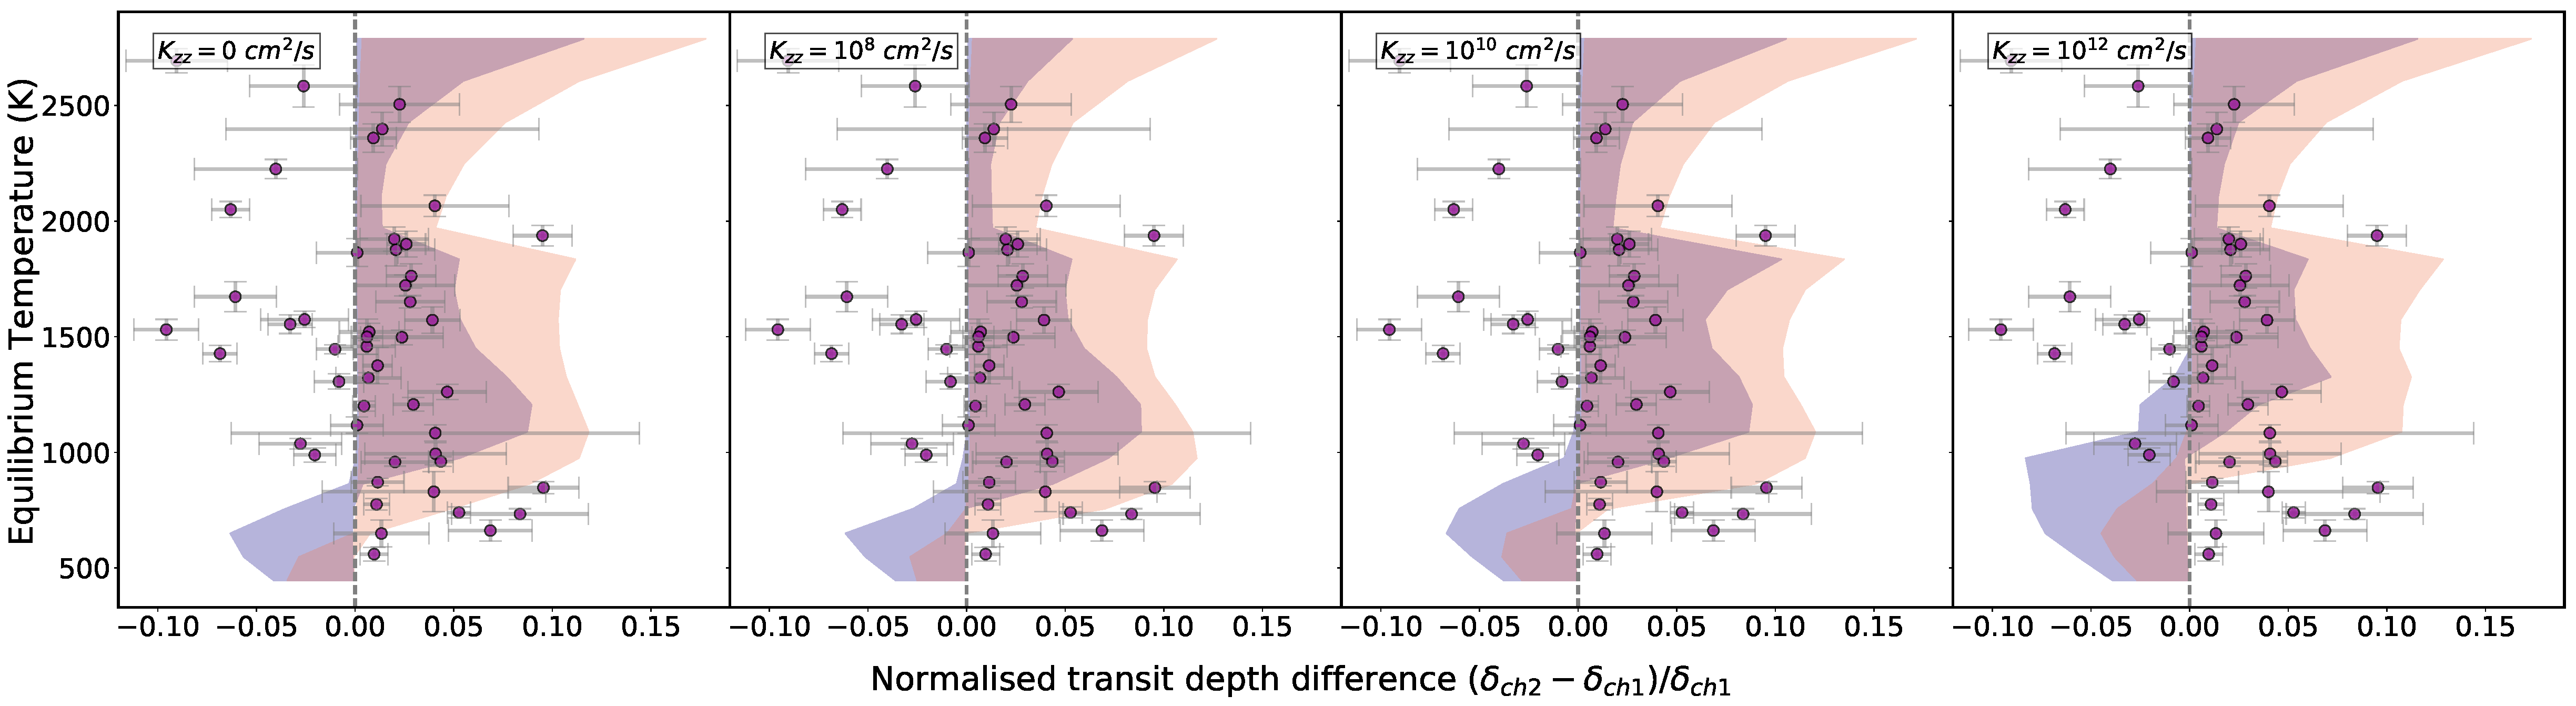
\includegraphics[width=\textwidth]{Kzzmodels.pdf}
%     \caption{Normalised \spitzer transit depth difference as a function of the equilibrium temperature for the full grid of transmission models created with PLATON (\citep{Zhang2019}, see Section \ref{P1:sec:PLATON}). Panels from left to right show no vertical mixing, Kzz = 1e8, Kzz = 1e10 and Kzz = 1e12. First row shows the 1x solar composition and second row shows the 30x solar composition. Gray dashed line represents a gray opacity source showing no spectral features.}
%     \label{P1:fig:Kzz}
% \end{figure*}

    % \item Shami models
%Heng 2014 equation
% \begin{equation}
% \begin{split}
% \bar{T}^4 =& \frac{T_{\rm int}^4}{4} \left[ \frac{1}{\epsilon_{\rm L}} + \frac{m}{\epsilon_{\rm L_3} \beta^2_{\rm L_0}} \left( \kappa_0 + \frac{\kappa_{\rm CIA} m}{2 m_0} \right) \right] \\
% &+ \frac{T_{\rm irr}^4}{8} \left[ \frac{1}{2 \epsilon_{\rm L}} + {\cal E}_2 \left( \frac{\kappa_{\rm S}}{\kappa_{\rm L} \beta_{\rm S_0}} - \frac{\kappa_{\rm CIA} m \beta_{\rm S_0}}{\epsilon_{\rm L_3} \kappa_{\rm S} m_0 \beta_{\rm L_0}^2} \right) \right.\\
% &\left.+ \frac{\kappa_0\beta_{\rm S_0}}{\epsilon_{\rm L_3} \kappa_{\rm S}\beta_{\rm L_0}^2} \left( \frac{1}{3} - {\cal E}_4 \right) + \frac{\kappa_{\rm CIA} \beta_{\rm S_0}^2}{\epsilon_{\rm L_3} \kappa_{\rm S}^2 m_0 \beta_{\rm L_0}^2} \left( \frac{1}{2} - {\cal E}_3 \right) \right].
% \end{split}
% \label{P1:eq:heng}
% \end{equation}
%     \item Mike models
%     \item Equilibrium chemistry vs non-equilibrium
%     \item Effect of the star/photochemistry
% \end{itemize}

\section{Exoplanet atmosphere diversity}

%From the first exoplanet discovery in

% \spitzer/Infrared Array Camera (IRAC) \citep[e.g.,]{Knutson2008, Line2014}, Hubble Space Telescope (HST)/Wide Field Camera 3 (WFC3) \citep[e.g.,][]{Kreidberg2015, Kreidberg2018b, Arcangeli2018}, HST/Space Telescope Imaging Spectrograph (STIS) \citep[e.g.,][]{Charbonneau2002}, and several ground based observatories \citep[e.g.,][]{Swain2010, Sing2011, Huitson2017}.

The last 30 years of exoplanet research has seen the field progress from the first exoplanet detection \citep{Mayor1995}, through to the detection of the first exoplanetary atmosphere \citep{Charbonneau2002} and to the cataloging of thousands of exoplanets \citep[e.g.,][]{Borucki2010, Batalha2013}). Having categorized these planets (e.g. hot Jupiters, warm-Neptunes, and terrestrial planets), the field currently focuses on assessing their characteristics using space and ground-based spectroscopy and photometry. We are now in a realm of comparative exoplanetology. This thesis comprises the largest survey of the emission of exoplanets as well as the largest survey in transmission with \textit{Spitzer}/IRAC. The following section will discuss some of the notable survey results from the literature.

% From the first exoplanet discovery in 1995 to the first measurement of at atmosphere with \spitzerIRAC in 2005 we are now in a realm of comparative exoplanetology.

%, ranging from %cool gas giants \citep{Wallack2019},
%warm-neptunes  to
%hot Jupiters .
%and with \citep{Heng2016}
%and ultra-hot Jupiters \citep{Baxter2020}.

\subsection{Looking at planet ensembles}

% Transmission surveys

\subsubsection{Transmission surveys}


In recent years, there have been several studies exploring the trends in HST/WFC3 transmission spectra of warm-Neptunes \citep{Crossfield2017} and hot Jupiters \citep{Stevenson2016a, Sing2016, Heng2016, Barstow2017, Fu2017, Tsiaras2018}. Notably, \citet{Sing2016} performed a survey of 10 transiting planets by combining thress instruments: HST/STIS (which probes the alkali lines and the Rayleigh slope), HST/WFC3 (which probes the 1.4~\um~ water feature), and \spitzerIRAC (which probes \ce{CH4} and CO). They find that their sample of hot Jupiters is extremely diverse, exhibiting a continuum from the clear to cloudy atmospheres, see Figure \ref{int:fig:singetal}. They define a metric based on the difference in the transit depth measured in the infrared vs the optical wavelengths. They note that it correlates with the spectral strength of the water feature, indicating that this metric can be used to classify similar objects.

Similarly, \citet{Stevenson2016b} creates a metric for measuring the strength of the water feature using HST/WFC3 spectra and finds that it strongly correlates with planet temperature. This implies that cooler atmospheres below 700K are likely to have dampened features due to clouds. Around the same time, \citet{Heng2016} creates a dimensionless cloudiness index for a sub-sample of 7 planets from \citet{Sing2016}. Their index is based on the sodium and potassium lines of these planets and thus probing smaller particles than the metric of \citet{Stevenson2016b}, yet they still find a tentative decreasing cloudiness trend with increasing equilibrium temperature. Additionally, \citet{Crossfield2017} studied a sample of 6 warm-Neptunes with HST/WFC3 observations and found a correlation with the spectral features and the equilibrium temperature suggesting more optically thick clouds at lower temperatures.


\begin{figure}
    \centering
    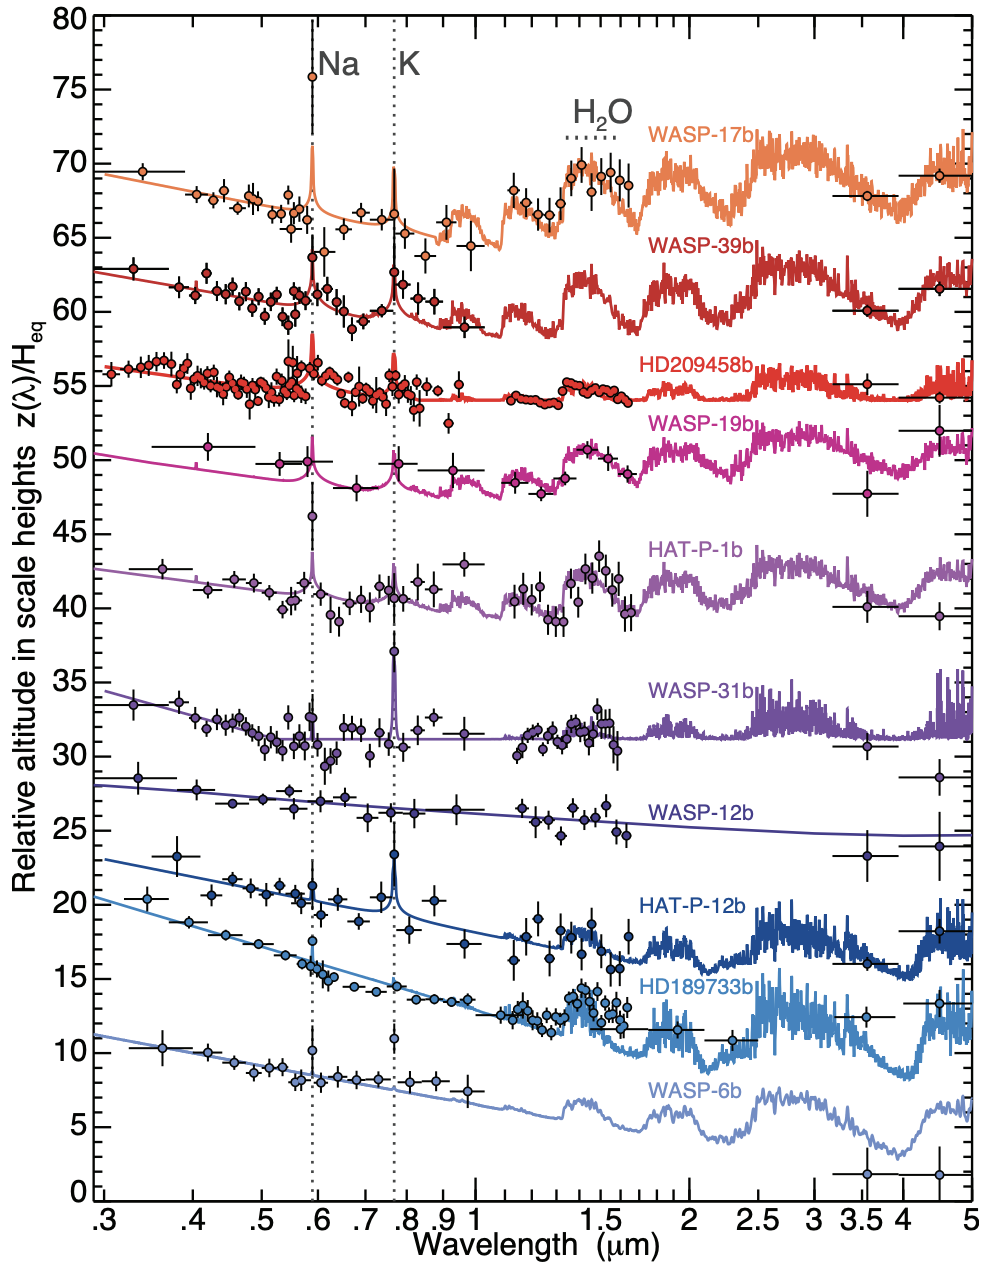
\includegraphics[width = \linewidth]{singetal.png}
    \caption{HST and \spitzer transmission spectra of 10 hot Jupiters. Solid colored lines show fitted atmospheric transmission spectra models where the alkali lines and the water feature are noted. The spectra are ordered in terms of their cloudiness, with the clear atmospheres appearing at the top of the image. The 3.6 and 4.5~\um~ \spitzerIRAC transit depths probe the \ce{CH4} and CO molecular features respectively. Image credit: \citet{Sing2016}}
    \label{int:fig:singetal}
\end{figure}

\citet{Barstow2017} performed a consistent retrieval of the 10 hot Jupiters presented in \citet{Sing2016}. They found that the planets between 1300-1700K are represented with deeper grayer clouds or clear atmospheres and the rest, cooler or hotter, are better with high altitude hazes causing Rayleigh scattering. And finally, \citet{Fu2017} collected all HST/WFC3 observations of 34 gas giants and compared them with a forward model for each planet calculated using Exo-Transmit. They found a negative slope in the absorption in scale heights vs equilibrium temperature which they attributed to decreasing cloudiness with increasing temperature.

Building on these works, in Chapter \ref{transits} we use the normalized difference between the two \spitzer infrared bandpasses to classify the chemical composition of the atmospheres of our sample. We tested how our metric correlates with all system parameters of the data and used it to compare our novel grids of forward models to the data. Finally, we incorporated important effects such as varying composition and disequilibrium chemistry into our modelling and compared the model grids with the data over a large range of system parameters.

\subsubsection{Emission surveys}

% Emission Surveys
There has also been a lot of work done studying the atmospheres of surveys of exoplanets by measuring the emission from their daysides. Despite the extreme differences in the amount of insolation they receive, hot Jupiters have similar equilibrium temperatures to late-type brown dwarfs. There have been several studies looking at the color-color and color-magnitude diagrams of exoplanets \citep{Triaud2014a, Triaud2014c, Dransfield2020, Melville2020}. \citet{Triaud2014c} calculate color-magnitude diagrams of a survey of 44 exoplanets using photometric distances and WISE magnitudes in combination with \spitzer emission in the four bandpasses (3.6, 4.5, 5.8, and 8.0~$\mu$m). Figure \ref{int:fig:triaud} displays the color-magnitude diagrams for the warm-\spitzer bandpasses. These figures show increasing scatter with increasing magnitude, which \citet{Triaud2014c} attributes to increased atmospheric diversity at colder temperatures. Furthermore, they found that hot Jupiters have colors similar to brown dwarf (MLT) colors i.e., these planets do not have simply featureless spectra in the infrared. However, it is likely that these similar colors are due to different processes in the atmospheres of hot Jupiters and brown dwarfs.

\begin{figure}
    \centering
    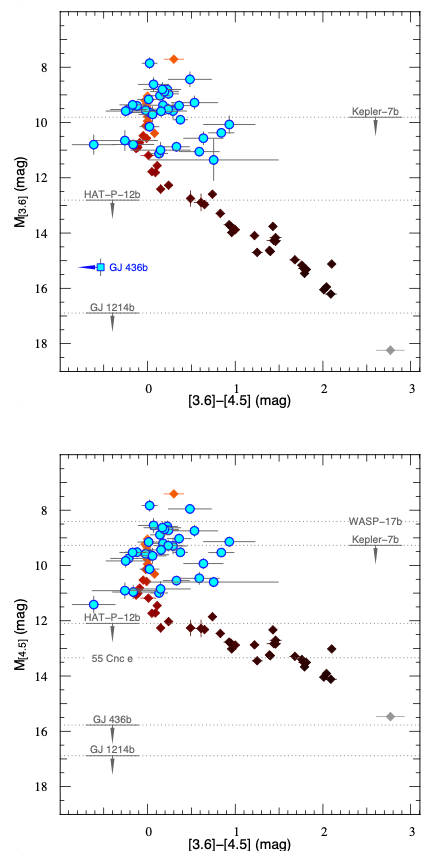
\includegraphics[height = 0.9\textheight]{triaud.png}
    \caption{Color-magnitude diagrams using the warm-\spitzer bandpasses. Blue dots show the planetary magnitudes and colors calculated from the secondary eclipse measurements. The colored diamonds show the magnitudes of ultra-cool brown dwarfs whose values were taken from \citet{Dupuy2012}. Image Credit: \citet{Triaud2014c}.}
    \label{int:fig:triaud}
\end{figure}

Additional studies have focused on using the infrared \spitzer emission observations to constrain the energy budgets of hot Jupiters. \citet{Schwartz2015} calculated the dayside effective temperature of a survey of 50 planets with thermal emission measurements in at least two infrared wavelengths (>0.8~$\mu$m). They compared the dayside effective temperature ($T_{\rm eff}$) with the irradiation temperature ($T_0$). If there is full redistribution of stellar irradiation then the effective dayside temperature will be the equilibrium temperature, where $T_{eq,\textit{0}} = (1/4)^{1/4} T_0 \approx 0.71T_0$. They found that the daysides of hotter planets deviate further from equilibrium temperature estimations, implying that the hotter planets do not redistribute heat as efficiently from their day to nightsides. This supports the previous claim by \citet{Cowan2011b} that the hottest planets have lower Bond albedo and/or less efficient heat transport, and is in agreement with theoretical predictions about redistribution efficiency in \citet{Perez-Becker2013}. However, \citet{Schwartz2017} incorporated phase offsets into their energy budget calculations of six planets. This pushed the results for these planets toward the lower Bond albedos scenario with slightly higher heat transport than previous measurements.

Furthermore, \citet{Garhart2020} performed a uniform analysis of 36 planets with \\
\spitzerIRAC secondary eclipses measured at 3.6 and 4.5~$\mu$m. They calculated the brightness temperatures and found an increasing trend in the brightness temperature ratio with equilibrium temperature. In Chapter \ref{eclipses}, we use these results in combination with 42 other planets with both 3.6 and 4.5~$\mu$m emission measurements to study how the dayside emission changes between the hot and the ultra-hot Jupiters. We revisit the trends seen in \citet{Schwartz2015} and \citet{Garhart2020} with our expanded survey of 78 planets in emission. When we carefully analyzed and calculated  the brightness temperatures, we found that the trend with dayside temperature and irradiation temperature is less significant than before. This was partially due to previous studies not incorporating a stellar model inplace of a blackbody for the star.
%Furthermore, typically the effective temperature is calculated by fitting a blackbody to the spectral energy distribution of the planet. In this case, there are just two photometric points, one of which has a strong CO emission feature (4.5~\um~). Therefore, calculating the effective temperature as a weighted mean of the two \spitzer brightness temperatures can bias the effective temperature results towards hotter temperatures. We suggest that the dayside effective temperature is better approximated with just the 3.6~\um~ brightness temperature, as this probes closer to the continuum. When this is done, the trend suggesting lower redistribution efficiency with hotter planets is no longer statistically significant. However, there remains a large scatter in the brightness temperatures of hotter planets compared to cooler planets, which could suggest a range of redistribution efficiencies for the hottest planets.
Additionally, in Chapter \ref{transits} we revisit the color-magnitude diagrams of \citet{Triaud2014b} with our expanded survey in combination with GAIA data release 2 distances and find that the larger sample is in agreement with previous works.

\subsection{The Ultra-hot Jupiters as a separate class}

Ultra-hot Jupiters are the newest class of exoplanets, it was only in the last few years that their atmospheres started to be understood \citep[e.g.,][]{Arcangeli2018, Parmentier2018b, Lothringer2018, Kitzmann2018}. Previously, emission spectra of these ultra-hot planets appeared to be blackbodies and the abundances retrieved from model fitting were very different from the general population of hot Jupiters \citep{Stevenson2014b, Haynes2015,Evans2017,Sheppard2017}. Retrieved abundances were driven in part by the strong CO feature seen with \spitzerIRAC and the lack of \ce{H2O} feature at the HST/WFC3 wavelengths. This combination resulted in high retrieved C/O ratios, which would have required most of the oxygen to be locked up in CO leaving very little to form \ce{H2O}. These high C/O ratios lead to questions regarding formation, why should the ultra-hot planets differ in metallicity from their cooler counterparts?

In \citet{Arcangeli2018} they explored the effect of molecular dissociation of molecules such as \ce{H2O} and TiO, as well as the recombination of H atoms with electrons to form H-. They found that when including these effects they were able to explain the emission spectra without the need to invoke very high metallicity (see Figure \ref{int:fig:w18}). The H- continuum opacity dominates the spectrum at the HST/WFC3 wavelengths and fills in the gap at 1.3~\um~while we see the bump of \ce{H2O} in emission at 1.5~\um, making the spectrum appear like a blackbody.

Furthermore, with TiO and VO dissociated on the dayside, there still remained temperature inversions in model atmospheres of ultra-hot Jupiters, which were due to the strong absorption of atomic metals (Fe, Mg, SiO) and metal hydrides such as FeH \citep{Lothringer2018}. Observations of temperature inversions in hot Jupiters were notoriously hard to find, with only hints of emission in the \spitzer bandpasses in a few planets \citep[e.g.,][]{Nymeyer2011, Deming2012}. However, there have now been a few observations of inversions in the ultra-hot Jupiters: WASP-33b, WASP-121b, and WASP-18b (Figure \ref{int:fig:w18}) \citep{Haynes2015, vonEssen2015, Evans2017, Arcangeli2018, Kreidberg2018b}. It is in this context that in Chapter \ref{eclipses} we look at how the dayside emission in the two \spitzer bandpasses changes as the temperature of the planets increases. We find a transition at around 1700K, which is likely caused by temperature inversions resulting in a strong CO feature appearing in emission.

As is mentioned in Section \ref{int:sec:variability}, the extreme atmospheres of ultra-hot Jupiters, in particular the high degree of ionization due to the intense stellar irradiation, could result in the dayside emission being variable in time. Additionally, the effects of dissociation and recombination of \ce{H2} were studied in \citet{Komacek2018b} and \citet{Bell2018}. It was discovered that recombination of atomic hydrogen occurs when it is transported from the hot dayside to the cooler nightside of these planets. This recombination releases a significant amount of heat that can warm up the nightside of the planet, increasing the global efficiency of heat redistribution \citep{Mansfield2020}. This result is in contrast with previous suggestions of lower efficiency of heat redistribution in the hottest planets and might be why we do not see this trend in the brightness temperatures measured in Chapter \ref{eclipses}. Additionally, dissociation, recombination and transport between the day and nightsides could also be a cause of the variability that we see in the dayside of WASP-18b in Chapter \ref{w18b}.

\subsection{The cool planets}

In this thesis (Chapters \ref{transits} and \ref{TTVs}), we also study some of the coolest gas giants that we know of, with temperatures around 500K. Cooler exoplanets have lower signal-to-noise ratio both in transmission and emission, making their atmospheres extremely difficult to characterize. There have been several studies focusing on the characterization of individual cool gas-giant exoplanets. Notably, the atmosphere of the Neptune mass planet, GJ436b, has been studied on many occasions in both emission and transmission with HST and \spitzerIRAC \citep{Deming2007, Demory2007, Gillon2007a, Gillon2007b, Stevenson2010a, Beaulieu2011, Knutson2011, Lanotte2014, Knutson2014a, Morley2017}. With an equilibrium temperature of 670K, chemical equilibrium models would predict that the atmosphere would have a high methane abundance, however, the atmosphere of GJ436b was shown to be substantially methane deficient \citep{Stevenson2010a, Knutson2011, Lanotte2014}. Furthermore, methane depletion compared to equilibrium chemistry expectations has been observed in many other warm giant planets with HST observations, e.g., WASP-107b and WASP-117 b \citep{Kreidberg2018a, Spake2018} or combined HST and \spitzer e.g., GJ3470 b \citep{Benneke2019}, HAT-P-11 b \citep{Chachan2019}, HAT-P-26 b \citep{Wakeford2017}, and WASP-39 b \citep{Wakeford2018}.

\citet{Kammer2015} performed a small uniform survey of 5 cool gas giant planets (HAT-P-19b, WASP-6b, WASP-10b, WASP-39b, WASP-67b) with \spitzerIRAC 3.6 and 4.5~\um. They found a tentative correlation in the brightness temperature ratio and planet mass. They did not discover a trend with the equilibrium temperature. However, in Chapter \ref{eclipses} we look for trends with the brightness temperature ratio againt equilibrium temperature for the whole sample of planets in emission, including those from \citet{Kammer2015}, and compare to models.
We do find a trend with equilibrium temperature and brightness temperature ratio throughout the entire range of temperatures. However, notably, the models also suggest that there is a trend with brightness temperature ratio and equilibrium temperature of the coolest planets. This trend is also highly dependent on the metallicity of the host star and can switch between being correlated when [M/H] = 1 to anti-correlated when [M/H] = -1, see Figure \ref{int:fig:Tbratio}. Furthermore, \citet{Wallack2019} present an analysis of 5 more cool gas giants (HAT-P-15b, HAT-P-17b, HAT-P-18b, HAT-P-26b, and WASP-69b) and find a tentative trend with \ce{CH4}/(CO +\ce{CO2}) ratio and stellar metallicity, which is in agreement with our models.

\begin{figure}
    \centering
    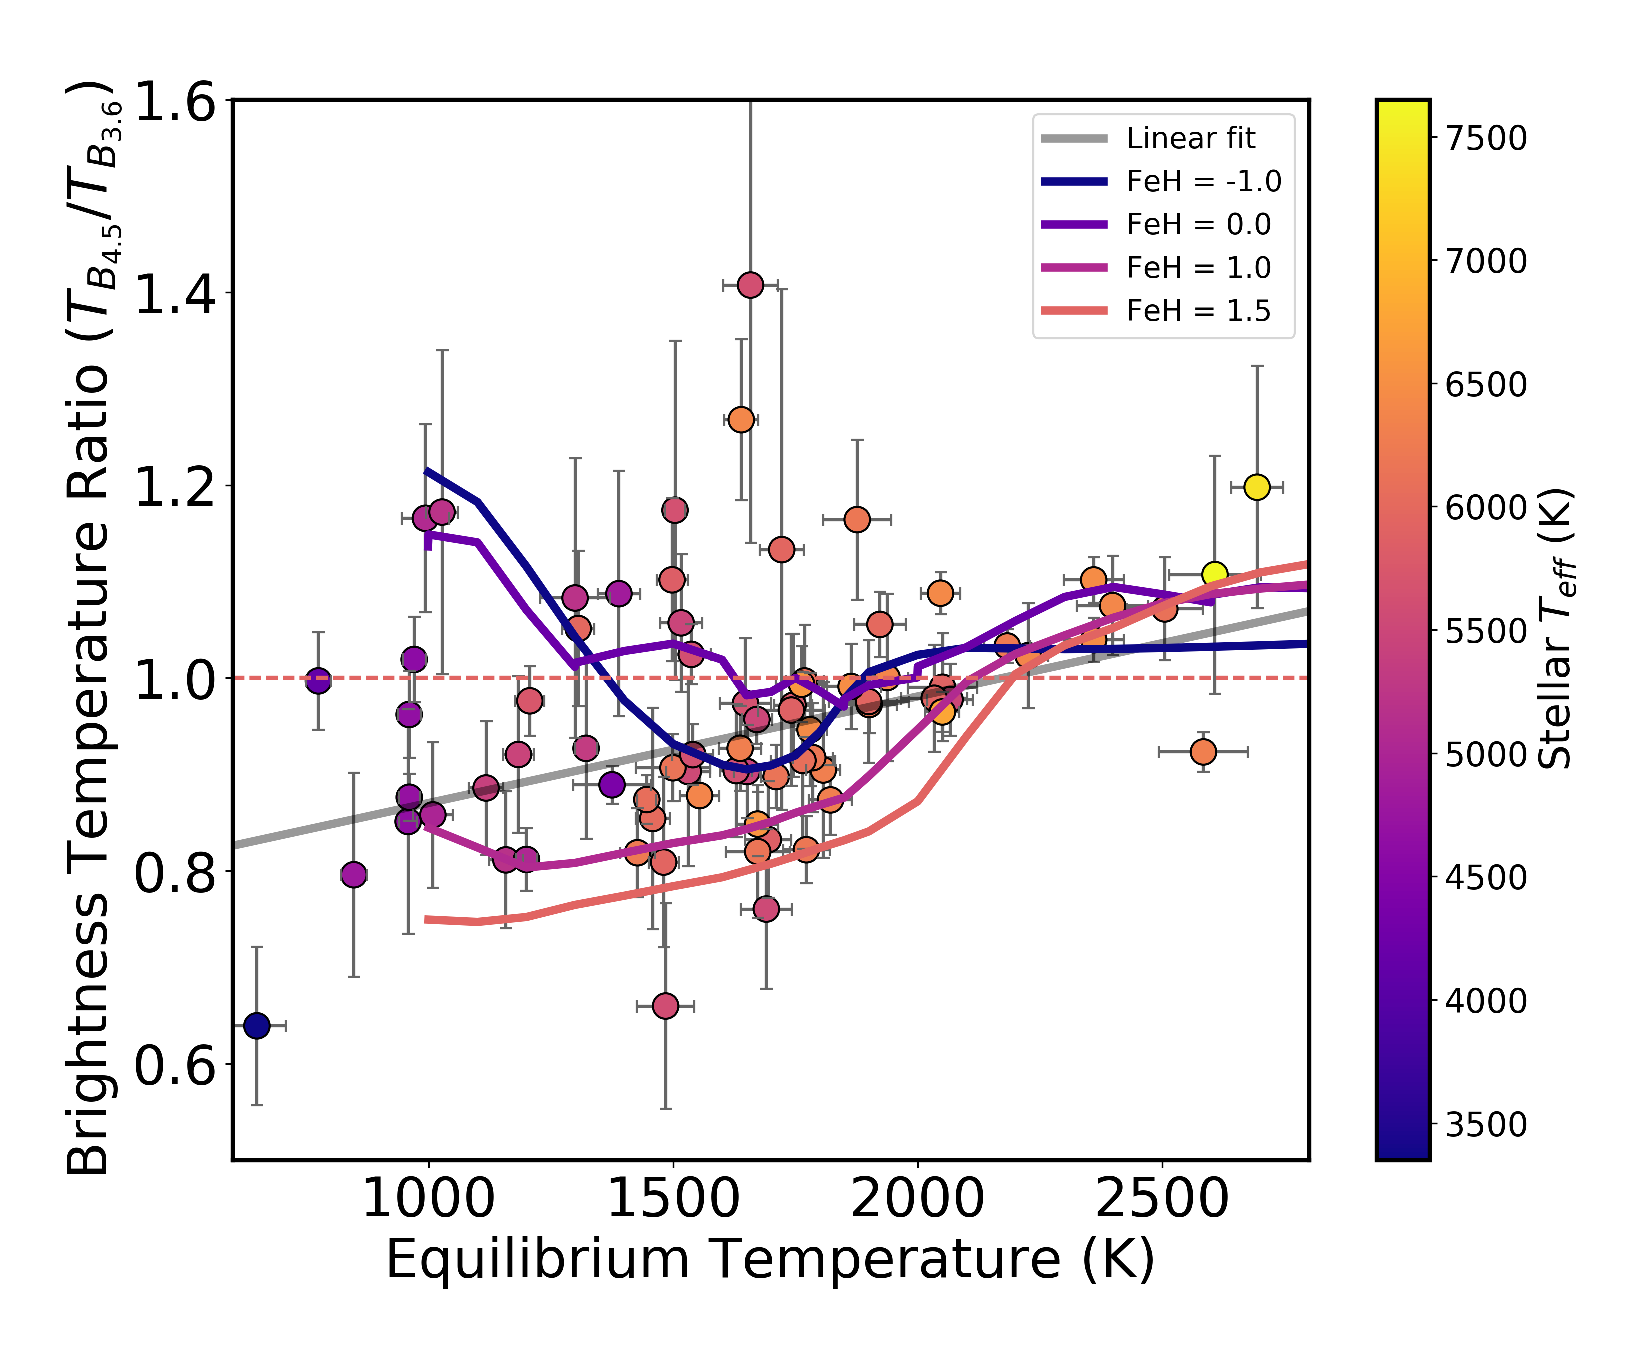
\includegraphics[width = \linewidth]{TbratiovsTeq_PHOENIX_intpl_wlabels.pdf}
    \caption{Brightness temperature ratio from \spitzerIRAC observations of our survey of 78 planets plotted against the equilibrium temperature. Remake of Figure 4 of Chapter \ref{eclipses} except the grids of models are not interpolated over all parameters, instead we show the tracks for the different metallicities of the host star, which is the largest contributing factor to the spread of the models. The different metallicities indicate both a positive and a negative correlation with ratio of brightness temperatures of the the coolest planets against their equilibrium temperature depending on host star metallicity. }
    \label{int:fig:Tbratio}
\end{figure}


Several theories have been discussed to explain the lack of methane in the coolest hot Jupiters: including using non-equilibrium photochemical models \citep{Line2011}, models with hydrogen depletion \citep{Hu2015}, invoking tidal heating due to high eccentricity \citep{Agundez2014} and finally, high metallicity models (230-1000x solar) \citep{Moses2013b}. Additionally, the trend of brightness temperature against mass from \citet{Kammer2015} and against stellar metallicity from \citet{Wallack2019} all suggest a link between the atmospheric composition and planetary formation scenarios.

Predictions based on the chemical composition of the protoplanetary disks suggest that planets formed close-in have low C/O ratios \citep[e.g.,][]{Oberg2011,Eistrup2018}. However, there has been evidence for planets having super-solar C/O ratios (C/O > 0.54) \citep[e.g.,][]{Lodders2004,Madhusudhan2011}. This has interesting implications for their formation scenarios. In Chapter \ref{eclipses}, we compare the sample of 78 planets in emission with a grid of models spanning different regions of parameter space. One of these parameters is the C/O ratio of the planetary atmosphere. We find that our sample of 78 planets statistically disfavors the models with high C/O ratios (C/O = 0.85).

% \subsection{Atmospheres as a tracer of formation}

% The atmospheres of all four of the Solar system gas giant planets have metallicities that are enhanced compared to the Sun. Spectroscopy of these atmospheres results in carbon abundances that show an enrichment factor of $\sim$4, 10, 80, and 80, for Jupiter, Saturn, Uranus, and Neptune, respectively. This was understood using the core accretion model of planetary formation \citep{Pollack1996} i.e. once a solid core reaches 10 earth masses this core will accrete solids and gas from the midplane of the protoplanetary disk. The local composition of this disk determines the atmospheric composition of the planet. Therefore, measuring the atmospheric abundances can help us constrain the chemistry, location and density of the disk where the planet formed \citep[e.g.,][]{Lodders2004,Oberg2011}.

% \citet{Oberg2011} suggested that the role of snow lines of \ce{H2O}, \ce{CO2} and CO can create distinct changes in the local carbon to oxygen ratio of the planet-forming disk, and therefore the C/O ratio of an exoplanet atmosphere can allow us to further distinguish between different formation locations and migration histories. \citet{Eistrup2018} shows a more complete picture by incorporating changes in the disk throughout its lifetime, yet distinct predictions on the C/O ratio based on radial distance and age are still expected. Based on these works, one would expect that planets formed close-in to have low C/O ratios, however, there has been evidence for planets having super-solar C/O ratios (C/O > 0.54) \citep[e.g.,][]{Lodders2004,Madhusudhan2011}, which could lead to questions about their formation scenarios. In Chapter \ref{} we compare the sample of 78 planets in emission with a grid of models spanning different regions of parameter space, one of these parameters is the C/O ratio of the planet atmosphere. We find that our sample of 78 planets statistically disfavours the models with high C/O ratios (C/O = 0.85).

% \section{Miscellaneous}

\section{This Thesis} %forward looking

This thesis focuses on the statistical characterization of exoplanet atmospheres in the infrared using the \spitzer Space Telescope.

Chapter \ref{transits} presents the data analysis pipeline used and augmented throughout the different chapters of this thesis. We reduce the data and simultaneously fit the transit parameters \citep[using Batman;][]{Kreidberg2015} with a pixel level decorrelation model and temporal ramp. We create an automated search through all of the parameter space to determine the optimum background correction, centroiding, and photometric methods for the reduction. We use the pipeline to uniformly analyse a survey of 49 planets in transmission at 3.6 and 4.5~\um. Using these two wavelengths, we then define a model-independent metric for characterizing the atmospheric composition (probing the relative abundance of \ce{CH4} and \ce{CO}). We search for statistical trends using this \spitzer metric as a function of other planetary and stellar parameters. We hone in on how the equilibrium temperature plays a role in determining the chemistry of the atmosphere and the strength of the \spitzer metric. Finally, we compare the entire survey to custom grids of forward models containing important disequilibrium chemistry and varying metallicities.

Chapter \ref{eclipses} presents a survey of 78 gas giant exoplanets in emission. Using the eclipse depths at 3.6 and 4.5~\um, we carefully calculate the brightness temperatures by integrating properly over the \spitzer spectral response functions and by including a PHOENIX model for the stellar flux. We search for trends in the brightness temperatures and define a new metric for characterizing the dayside emission of the planets, called the deviation from a blackbody. Using this metric, we compare the sample to a comprehensive grid of self-consistent forward models, which contain temperature inversions and important phenomena for the ultra-hot Jupiters. Additionally, we alter our custom pipeline to analyse secondary eclipses and we analyse the hottest ultra-hot Jupiter known, KELT-9b, and comment on how this planet fits into the population.

Chapter \ref{w18b} presents a focused look at one ultra-hot exoplanet in particular, WASP-18b. Using our custom data analysis pipeline, we analyse 10 almost consecutive eclipses at 4.5~\um. We find a periodic signal in the brightness variability in time. We confirm the signal by performing different analyses of the data and then explore possible physical phenomena that could be responsible for a time variable brightness in the atmosphere.

Finally, Chapter \ref{TTVs} presents an analysis of seven of the coolest planets from our science exploration program. These planets are part of three multi-planet systems (Kepler-9, Kepler-18 and Kepler-32) and one circumbinary system (Kepler-16). Due to the low signal-to-noise of the multi-planet system planets, we alter the pipeline to extract only the transit times. We then compare the measured transit times to predictions made with timing variation models based on the original Kepler observations, which can help pin down the planetary masses. On the other hand, the signal-to-noise ratio of the Kepler-16b data is high, allowing us to extract exquisite transit lightcurves and to fit for the full range of transit parameters. We make predictions using a photo-dynamical model of the Kepler-16 system and compare this to the 3.6 and 4.5~\um transit lightcurves.

%%% Local Variables:
%%% mode:latex
%%% TeX-master: "../../thesis_renzo"
%%% End:
